% !TEX root = ../main/main.tex
% chapter_2_lit_review.tex
\chapter{Literature Review and Methodological Foundations}
\label{chap:litreview}

\paragraph{Methodology roadmap.} We organize this review into six methodological tiers that mirror the dissertation's hybrid architecture: (i) foundational models establishing the statistical basis for sports prediction; (ii) distributional modeling for scores, margins, and their dependence structure; (iii) machine learning methods including gradient boosting, ensemble theory, and feature attribution; (iv) evaluation and calibration frameworks for probabilistic forecasts; (v) decision theory connecting predictions to optimal wagering; and (vi) emerging methods from deep learning and causal inference. This structure emphasizes the complementary roles of interpretable generative models and flexible discriminative methods, unified by rigorous uncertainty quantification.

%=============================================================================
% TIER 1: FOUNDATIONAL MODELS
%=============================================================================
\section{Foundational Models for Sports Prediction}
\label{sec:foundations}

We situate the dissertation within a tradition of statistical modeling for sports outcomes, beginning with seminal works that established core concepts still central to modern approaches.

\subsection{Harville (1980): Linear-Model Predictions for NFL}
\label{subsec:harville1980}

\sdesc{Proposes linear models for NFL game outcomes, connecting team strengths and covariates to score differential and win probability.}

\mdesc{Let $M_{ij}$ be margin (home $i$ vs away $j$). A two-way design with home advantage $h$ and team effects $\theta_k$ reads}
\begin{equation}\label{eq:harville}
M_{ij} = h + (\theta_i - \theta_j) + \varepsilon,\qquad \varepsilon\sim \mathcal N(0,\sigma^2),
\end{equation}
estimated by (generalized) least squares, with identifiability constraints (e.g., $\sum_k \theta_k=0$). Win probability maps via $\Pr(M_{ij}>0)=\Phi\big((h+\theta_i-\theta_j)/\sigma\big)$.

\appdesc{Equation \eqref{eq:harville} is a baseline for spread pricing and win probability, and underlies state-space generalizations developed in \Cref{chap:methods}. The linear-Gaussian structure enables rapid weekly updates while providing interpretable team strength estimates that serve as priors for more complex models.}

\bridge{Margins provide a continuous target; the next step relates posted spreads to win probability so we can compare generative models with market quotes.}

\subsection{Stern (1991): Spread-to-Win Mapping}
\label{subsec:stern1991}

\sdesc{Relates posted spreads to win probability under a Gaussian margin model.}

\mdesc{With margin $M\sim\mathcal N(\mu,\sigma^2)$ and spread $p$, we obtain}
\begin{equation}\label{eq:stern-win}
\Prob(\text{favorite wins})=\Prob(M>0)=\Phi\!\Big(\frac{\mu}{\sigma}\Big),\qquad
\Prob(\text{favorite covers})=\Phi\!\Big(\frac{\mu-p}{\sigma}\Big).
\end{equation}

\appdesc{Empirical $\hat\sigma$ by era links spreads to win odds, and provides a consistency check for classifiers trained on features plus prices. The mapping enables translation between spread-based and moneyline-based evaluation metrics.}

\bridge{Knowing how spreads map to win odds, we next ask how team strengths evolve over time, motivating state-space ratings.}

\subsection{Glickman \& Stern (1998): State-Space Team Ratings}
\label{subsec:glickman1998}

\sdesc{Time-evolving team strengths with linear-Gaussian state evolution, estimated via Kalman filtering/smoothing.}

\mdesc{For team $k$ strength $\theta_{k,t}$,}
\begin{align}
\theta_{k,t} &= \theta_{k,t-1}+\eta_{k,t}, & \eta_{k,t}&\sim \mathcal N(0,\tau^2),\\
M_t &= h + (\theta_{h(t),t}-\theta_{a(t),t}) + \epsilon_t, & \epsilon_t&\sim \mathcal N(0,\sigma^2),
\end{align}
with standard Kalman recursions for posterior means/variances.

\appdesc{Supplies temporally stable latent strengths, yielding calibrated priors for spread/win models and robust inputs to score-distribution layers. The state-space formulation naturally handles missing data and provides uncertainty estimates that propagate through downstream predictions.}

\bridge{Margins summarize outcomes, but pricing totals and correlated bets needs a score model. Before introducing Poisson scoring, we survey methodological contributions from other major sports that inform our approach.}

\subsection{Cross-Sport Methodology Transfer}
\label{subsec:cross-sport}

Sports analytics methodology transcends individual sports. We highlight foundational contributions from baseball, basketball, and hockey whose concepts transfer directly to NFL prediction.

\paragraph{Baseball: Sabermetrics and expected value.} Baseball's sabermetric revolution, pioneered by \citet{james1982} and formalized by \citet{tango2007book}, established core principles now universal in sports analytics: (i) decomposing outcomes into skill and luck components, (ii) regressing observed performance toward population means, and (iii) weighting events by their run/point expectancy. The run expectancy matrix---expected runs scored from each base-out state---directly inspired Expected Points Added (EPA) in football \citep{burke2009epa}. \citet{albert2003curve} demonstrated Bayesian hierarchical models for player evaluation, a framework we adopt for team strength estimation.

\paragraph{Basketball: Player impact and plus-minus.} \citet{rosenbaum2004measuring} introduced adjusted plus-minus (APM), using regression to isolate individual player contributions from team and opponent effects. \citet{engelmann2017rpm} refined this into Regularized APM (RAPM) with ridge regression to handle collinearity among teammates. These methods inform our opponent-adjusted features: just as APM separates player skill from lineup context, we separate team performance from schedule difficulty. \citet{cervone2016multiresolution} developed Expected Possession Value (EPV), a continuous-time analog of EPA that values each moment of a possession---a framework applicable to NFL drive modeling.

\paragraph{Hockey: Expected goals and low-scoring dynamics.} \citet{macdonald2012expected} formalized expected goals (xG) models for hockey, estimating goal probability from shot location, type, and game state. Like the Poisson models we discuss next, hockey's low-scoring nature (2--3 goals per team) demands distributional modeling of outcomes. \citet{thomas2013competing} applied competing hazard models to player ratings, handling the discrete events (goals, assists) that punctuate continuous play---conceptually similar to how we model scoring drives within NFL games.

\paragraph{Synthesis.} These cross-sport contributions share common themes: (i) context adjustment (opponent, venue, game state), (ii) expectation-based valuation (run expectancy, EPA, xG, EPV), (iii) shrinkage toward priors for small samples, and (iv) decomposition of team outcomes into individual contributions. We draw on all four themes throughout this dissertation.

\bridge{With this cross-sport foundation established, we now introduce Poisson scoring models---developed for soccer but applicable across sports with discrete scoring.}

\subsection{Maher (1982): Poisson Score Model}
\label{subsec:maher1982}

\sdesc{Independent Poisson scoring intensities by team/venue, developed for soccer but foundational for all sports score modeling.}

\mdesc{$X\sim\mathrm{Pois}(\lambda)$, $Y\sim\mathrm{Pois}(\mu)$ with log-links $\log\lambda = \alpha_i+\beta_j+v_{\text{home}}$, $\log\mu=\alpha'_j+\beta'_i$.}

\appdesc{Although developed for soccer (where typical scores are 1--3 goals), the Poisson framework transfers to NFL with higher intensity parameters. The resulting Skellam margin (\Cref{subsec:skellam-mom}) remains useful for integer margins, teaser/middle pricing, and key-number analysis. The Poisson assumption provides a generative foundation that extends naturally to bivariate and dynamic settings.}

\bridge{Independent Poisson can misfit low scores; Dixon--Coles shows how to correct dependence near small counts.}

\subsection{Dixon \& Coles (1997): Dependence and Low-Score Adjustments}
\label{subsec:dixon1997}

\sdesc{Soccer betting market model with Poisson adjustments for low-score dependence and time-decay weighting.}

\mdesc{Likelihood reweighting for small-score outcomes modifies a baseline Poisson log-likelihood. Let $\rho$ control dependence for $(x,y)\in\{0,1\}^2$:}
\begin{equation}
\Pr(X=x,Y=y) = \tau_{\lambda,\mu}(x,y)\cdot\frac{\lambda^x e^{-\lambda}}{x!}\cdot\frac{\mu^y e^{-\mu}}{y!},
\end{equation}
where $\tau$ is an adjustment factor near unity that corrects for under/overdispersion at low scores.

\appdesc{While the low-score adjustment is soccer-specific (0--0 and 1--1 draws are common), the time-decay weighting transfers directly to NFL: recent games should receive more weight than distant ones. This addresses the non-stationarity inherent in sports data and motivates our era-aware feature engineering.}

\bridge{Fixing low-score dependence still assumes independent team scores; next we model positive score correlation via a shared component.}

\subsection{Karlis \& Ntzoufras (2003): Bivariate Poisson}
\label{subsec:karlis2003}

\sdesc{Soccer score model with shared latent component for positively correlated team scores.}

\mdesc{$X=U+Z$, $Y=V+Z$ with $U,V,Z\overset{\text{iid}}\sim\mathrm{Pois}(\cdot)$; then $\mathrm{Cov}(X,Y)=\E[Z]=\lambda_0$. The joint pmf admits closed form via trivariate Poisson sums.}

\appdesc{The bivariate Poisson structure transfers to NFL for modeling correlated scoring (pace, situational exchanges) and yields coherent joint pricing for same-game parlays. The shared component $\lambda_0$ models game-level factors (weather, tempo) that affect both teams---equally relevant in football codes.}

\bridge{Correlation and intensities vary through the season; the dynamic bivariate Poisson extends these ideas over time.}

\subsection{Koopman, Lit \& Lucas (2015): Dynamic Bivariate Poisson}
\label{subsec:koopman2015}

\sdesc{English Premier League model with time-varying attack/defense parameters in a state-space framework.}

\mdesc{Let $\lambda_{i,t}=\exp(x_{i,t}^\top\beta + s_{i,t})$ with latent $s_{i,t}$ following an AR(1); similarly for $\mu_{j,t}$ and a shared $\lambda_{0,t}$. Filtering uses simulation-based methods (e.g., particle filters).}

\appdesc{The state-space formulation for evolving team strengths transfers directly to NFL, where team quality varies within and across seasons due to injuries, trades, and scheme changes. The time-varying dependence structure improves same-game parlay risk estimates by capturing temporal evolution in scoring rates.}

\bridge{For margin-centric pricing and key-number analysis we also need a direct model for integer differences: enter the Skellam distribution.}

\subsection{Skellam (1946): Difference of Two Poissons}
\label{subsec:skellam1946}

\sdesc{Closed-form pmf for $D=X-Y$ with $X,Y$ independent Poisson; moments and generating functions.}

\mdesc{See \eqref{eq:skellam-pmf}--\eqref{eq:skellam-moments}; mgf $M_D(t)=\exp\big(\lambda(e^t-1)+\mu(e^{-t}-1)\big)$.}

\appdesc{Natural integer-margin model; a convenient substrate for key-number reweighting and teaser/middle pricing. The Skellam distribution provides the theoretical basis for margin probability calculations throughout the dissertation.}

\bridge{Orthogonal decomposition of features enables pure signal extraction. We formalize this principle next via the Frisch-Waugh-Lovell theorem.}

\subsection{Frisch-Waugh-Lovell Theorem: Orthogonal Feature Decomposition}
\label{subsec:fwl-theorem}

\sdesc{Establishes equivalence between partial regression coefficients and residual-on-residual regression, foundational for orthogonalization methodologies.}

\mdesc{Consider regression of $Y$ on $X_1$ and $X_2$:}
\begin{equation}
Y = \beta_1 X_1 + \beta_2 X_2 + \epsilon.
\end{equation}
The Frisch-Waugh-Lovell theorem \citep{frisch1933,lovell1963} states that $\hat{\beta}_2$ (partial regression coefficient) is identical to coefficient from residual regression:
\begin{align}
\tilde{Y} &= Y - \hat{Y}_{X_1}, \quad \text{where } \hat{Y}_{X_1} = \text{proj}_{X_1}(Y), \\
\tilde{X}_2 &= X_2 - \hat{X}_{2,X_1}, \quad \text{where } \hat{X}_{2,X_1} = \text{proj}_{X_1}(X_2), \\
\tilde{Y} &= \hat{\beta}_2 \tilde{X}_2 + \tilde{\epsilon}.
\end{align}
Here $\tilde{Y}$ is $Y$ orthogonalized with respect to $X_1$, and $\tilde{X}_2$ is $X_2$ orthogonalized with respect to $X_1$. The residual regression coefficient $\hat{\beta}_2$ equals the partial regression coefficient from joint regression.

\appdesc{Motivates two-stage residual architectures that decompose predictions into opponent-orthogonal components. Feature orthogonalization can eliminate confounding more effectively than complex models on raw features, as demonstrated in our Ridge Residuals methodology (\Cref{chap:methods}).}

\bridge{Orthogonal decomposition enables pure signal extraction from confounded data. Next we address calibration assessment via proper scoring rules.}

%=============================================================================
% TIER 2: DISTRIBUTIONAL MODELING
%=============================================================================
\section{Distributional Modeling for Scores and Margins}
\label{sec:distributions}

This section develops the mathematical machinery for modeling score and margin distributions, which underpin spread, total, and teaser pricing.

\subsection{Skellam Distribution: Construction and Moments}
\label{subsec:skellam-mom}

The Skellam distribution \citep{skellam1946} arises as the difference of two independent Poisson variates and underpins integer margin modelling. Early association football (soccer) score models \citep{maher1982,dixon1997} adopt Poisson assumptions to capture low-scoring regimes; extensions to allow dependence \citep{karlis2003,koopman2015} are crucial for joint pricing of spreads and totals. Although developed for soccer, the mathematical framework---bivariate Poisson, Skellam margins, dependence correction---transfers directly to NFL prediction with appropriate reparameterization for higher scoring rates.

Let $X\sim\mathrm{Pois}(\lambda)$ and $Y\sim\mathrm{Pois}(\mu)$ independent. The difference $D=X-Y$ has the Skellam pmf
\begin{equation}\label{eq:skellam-pmf}
\Prob(D=d)=e^{-(\lambda+\mu)}\!\left(\frac{\lambda}{\mu}\right)^{d/2}
\,I_{|d|}\!\big(2\sqrt{\lambda\mu}\big),\qquad d\in\mathbb{Z},
\end{equation}
with $I_\nu(\cdot)$ the modified Bessel function of the first kind. Using pgfs and coefficient extraction yields \eqref{eq:skellam-pmf}. Its mean/variance are
\begin{equation}\label{eq:skellam-moments}
\E[D]=\lambda-\mu,\qquad \Var(D)=\lambda+\mu.
\end{equation}
It is often convenient to reparametrize by $(\mu_D,\sigma_D^2)=(\lambda-\mu,\lambda+\mu)$ with $\lambda=\tfrac12(\sigma_D^2+\mu_D)$ and $\mu=\tfrac12(\sigma_D^2-\mu_D)$.

\paragraph{Gaussian limit.} For large $(\lambda,\mu)$ with fixed $(\mu_D,\sigma_D^2)$, the Skellam distribution approaches $\mathcal{N}(\mu_D,\sigma_D^2)$, motivating probit links between spreads and win probability. This justifies the Gaussian approximations in \Cref{subsec:stern1991} for typical NFL scoring rates.

\subsection{Bivariate Poisson: PMF, Likelihood, and EM Updates}
\label{subsec:bp-pmf}

Following \Cref{subsec:karlis2003}, write scores as $X=U+Z$, $Y=V+Z$ with independent $U\sim\mathrm{Pois}(\lambda_1)$, $V\sim\mathrm{Pois}(\lambda_2)$, $Z\sim\mathrm{Pois}(\lambda_0)$. Then
\begin{align}
\Pr(X=x,Y=y)
&= e^{-(\lambda_0+\lambda_1+\lambda_2)}\sum_{z=0}^{\min(x,y)} \notag\\[-2pt]
&\quad \tfrac{\lambda_0^z}{z!}\,\tfrac{\lambda_1^{x-z}}{(x-z)!}\,\tfrac{\lambda_2^{y-z}}{(y-z)!},\label{eq:bp-pmf}\\[-2pt]
\Cov(X,Y) &= \lambda_0,\quad \E[X]=\lambda_0+\lambda_1,\quad \E[Y]=\lambda_0+\lambda_2.
\end{align}
For observations $\{(x_i,y_i)\}$ the log-likelihood is $\ell(\boldsymbol\lambda)=\sum_i \log \Pr(X=x_i,Y=y_i)$ with \eqref{eq:bp-pmf}. A convenient EM arises by treating $Z_i\sim\mathrm{Pois}(\lambda_0)$ as latent:
\begin{align}
\text{E-step: } &\ w_{i,z}=\Pr(Z_i=z\mid x_i,y_i;\boldsymbol\lambda) \propto \notag\\[-2pt]
&\quad \tfrac{\lambda_0^z}{z!}\,\tfrac{\lambda_1^{x_i-z}}{(x_i-z)!}\,\tfrac{\lambda_2^{y_i-z}}{(y_i-z)!},\label{eq:bp-weights}\\
\text{M-step: } &\ \lambda_0^{\text{new}}=\frac{1}{n}\sum_i \sum_{z=0}^{m_i} z\,w_{i,z},\notag\\[-2pt]
&\ \lambda_1^{\text{new}}=\frac{1}{n}\sum_i \sum_{z=0}^{m_i} (x_i-z)\,w_{i,z},\notag\\[-2pt]
&\ \lambda_2^{\text{new}}=\frac{1}{n}\sum_i \sum_{z=0}^{m_i} (y_i-z)\,w_{i,z},
\end{align}
where $m_i=\min(x_i,y_i)$. In practice we maximize the conditional expectation of the complete-data log-likelihood.

\paragraph{Toy numeric.} For $(x,y)=(2,1)$ and $(\lambda_0,\lambda_1,\lambda_2)=(0.3,1.4,1.1)$,
\[\Pr(X=2,Y=1)=e^{-2.8}\Big(\tfrac{\lambda_0^0\lambda_1^2\lambda_2^1}{2!1!}+\tfrac{\lambda_0^1\lambda_1^1\lambda_2^0}{1!1!0!}\Big)\approx e^{-2.8}\,(1.078+0.42)\approx 0.216,\]
illustrating the latent $Z$ mixing across $z=0,1$.

\subsection{Stern's Spread-to-Win Map: Full Derivation}
\label{subsec:stern-derivation}

We connect posted spreads to win probabilities following \citet{stern1991}, which motivates probit links in baseline classifiers. Assume the realized margin $M$ satisfies $M=\mu+\varepsilon$ with $\varepsilon\sim\mathcal{N}(0,\sigma^2)$. If the posted spread is $p$ (favorite $-p$), then
\begin{equation}\label{eq:stern-win-full}
\Prob(\text{favorite wins})=\Prob(M>0)=\Phi\!\Big(\frac{\mu}{\sigma}\Big),\qquad
\Prob(\text{favorite covers})=\Phi\!\Big(\frac{\mu-p}{\sigma}\Big).
\end{equation}
\begingroup\sloppy
Under efficiency for the mean $\mu\approx p$ we get the classical approximation $\Prob(\text{win})\approx\Phi(p/\sigma)$. Empirically we estimate $\sigma$ with a probit regression of win indicators on posted spreads; we report $\hat\sigma$ by season/era in \Cref{chap:data}.
\endgroup

\begin{example}[Worked mapping]
If the market posts $p=3$ and historical fit yields $\hat\sigma=13.5$, then Stern's map gives $\Pr(\text{win})\approx\Phi(3/13.5)\approx 0.59$. The implied moneyline fair odds are roughly $1/0.59\approx1.69$ (decimal), before vig and correlation adjustments.
\end{example}

\subsection{Key-Number Reweighting as Constrained Projection}
\label{subsec:key-reweight}

NFL margins concentrate on \emph{key integers} (3, 6, 7, 10) due to scoring mechanics. Rather than reweight small \emph{scores} as in Dixon--Coles, we reweight the \emph{margin pmf} $q(d)$ multiplicatively to match empirical key masses while preserving location/scale.

Let $q(d)$ be a baseline integer pmf (Skellam or discretized Gaussian) for the margin $D$ and let $\mathcal{K}=\{3,6,7,10\}$. We seek nonnegative weights $\{w_d\}$ s.t.\ $\tilde q(d)=w_d q(d)$ is a pmf matching empirical key masses $\{m_k\}_{k\in\mathcal{K}}$:
\begin{align}\label{eq:reweight-ls}
\min_{\{w_d\ge0\}} \quad & \sum_{k\in\mathcal{K}} \big(w_k q(k)-m_k\big)^2 \\
\text{s.t.}\quad &
\sum_{d} w_d q(d)=1,\quad
\sum_d d\,w_d q(d)=\mu_D,\quad
\sum_d (d-\mu_D)^2 w_d q(d)=\sigma_D^2. \nonumber
\end{align}

The last two constraints preserve mean/variance so reweighting changes shape, not location/scale. In matrix form, \eqref{eq:reweight-ls} is a small convex QP; if only normalization and key masses are imposed it has a closed form via Lagrange multipliers.

\paragraph{Practical effect.} In practice, this means the model assigns more realistic probability mass to key margins. For example, if the baseline puts only 12\% on a 3-point margin, the reweighted $\tilde q$ may allocate 18\% based on observed pushes. This directly improves expected value for teaser bets that cross 3 (and 7), because pricing reflects the higher chance of landing on those integers.

\paragraph{Feasibility and fallback.} The moment constraints imply a feasibility region for the target masses $\{m_k\}$. When empirical masses are extreme (e.g., unusually high mass at 3), \eqref{eq:reweight-ls} can be infeasible. We therefore (i) project $\{m_k\}$ onto the nearest feasible set and (ii) fall back to KL-tilting (\Cref{subsec:key-kl}) when needed.

\paragraph{Convergence and complexity.} For the projected-update routine (\Cref{alg:key-reweight}), the objective $\sum_{k\in\mathcal K}(w_k q(k)-m_k)^2$ is convex in $w$, and the projection onto linear moment constraints is nonexpansive; with a fixed step size $\eta\in(0,2/L)$ where $L=\max_k 2 q(k)^2$, the sequence of objective values decreases monotonically and converges to the minimum over the feasible set. Each iteration costs $O(|\mathcal{K}|+|\mathrm{supp}(q)|)$.

\begin{algorithm}[t]
  \caption{Key-number reweighting via projected updates}
  \label{alg:key-reweight}
  \begin{algorithmic}[1]
    \Require baseline pmf $q(d)$ on $\mathbb{Z}$; key set $\mathcal{K}$ with targets $m_k$; target moments $(\mu_D,\sigma_D^2)$; step size $\eta$
    \State initialize $w_d\leftarrow 1$ for all $d$; repeat for $T$ iters
    \State gradient on keys: for $k\in\mathcal{K}$, \; $g_k \leftarrow 2\big(w_k q(k)-m_k\big)\,q(k)$; set $g_d\leftarrow 0$ otherwise
    \State gradient step: $w_d \leftarrow \max\{0,\; w_d - \eta g_d\}$
    \State project to constraints: solve for multipliers $(\alpha,\beta,\gamma)$ s.t.\
      $\sum_d w_d q(d)=1$, $\sum_d d\,w_d q(d)=\mu_D$, $\sum_d (d-\mu_D)^2 w_d q(d)=\sigma_D^2$;
      update $w_d \leftarrow \max\{0,\; w_d + \alpha + \beta d + \gamma (d-\mu_D)^2\}$
    \State \textbf{until} convergence of $\sum_{k\in\mathcal{K}}|w_k q(k)-m_k|$
    \State \Return reweighted pmf $\tilde q(d)=w_d q(d)$
  \end{algorithmic}
\end{algorithm}

\paragraph{KL-tilting alternative (maximum entropy).}\label{subsec:key-kl}
An alternative with strong existence/positivity guarantees is multiplicative tilting that minimizes KL divergence to $q$:
\begin{align*}
\min_{\tilde q}\quad & \sum_d \tilde q(d)\log\frac{\tilde q(d)}{q(d)}\\
\text{s.t.}\quad & \sum_d \tilde q(d)=1,\ \sum_d d\,\tilde q(d)=\mu_D,\ \sum_d (d-\mu_D)^2\tilde q(d)=\sigma_D^2,\ \tilde q(k)=m_k\ (k\in\mathcal{K}).
\end{align*}
By convex duality, the solution has exponential form
\[
\tilde q_\alpha(d)\propto q(d)\exp\{\alpha_0+\alpha_1 d+\alpha_2 (d-\mu_D)^2+\sum_{k\in\mathcal{K}}\delta_k\,\mathbb{1}\{d=k\}\},
\]
with multipliers $\alpha,\delta$ found by Newton or projected gradient on the dual.

\subsection{Spread--Total Dependence via Copulas}
\label{subsec:copula-st}

We model dependence between margin $M$ and total $T$ to price correlated legs coherently. A convenient baseline is the \emph{Gaussian copula} \citep{nelsen2006}: $(Z_1,Z_2)\sim \mathcal{N}(\mathbf 0,\begin{psmallmatrix}1&\rho\\ \rho&1\end{psmallmatrix})$, set $(U,V)=(\Phi(Z_1),\Phi(Z_2))$, then $(M,T)=\big(F_M^{-1}(U),F_T^{-1}(V)\big)$. The joint exceedance for teaser legs $A=\{M>p_1\}$, $B=\{T>q_1\}$ is
\[
\Prob(A\cap B)=\iint 1\!\{F_M^{-1}(u)>p_1,\ F_T^{-1}(v)>q_1\}\,c_\rho(u,v)\,\dd u\,\dd v,
\]
with density $c_\rho$. For Gaussian copulas, Kendall's $\tau$ and $\rho$ relate by $\tau=\tfrac{2}{\pi}\arcsin(\rho)$, which we use to estimate $\rho$ robustly from rank correlation.

\paragraph{Tail behavior and $t$-copulas.} Gaussian copulas have \emph{zero tail dependence}, potentially understating joint tail risk for extreme margins/totals. A heavier-tailed alternative is the \emph{$t$-copula} with correlation $\rho$ and degrees of freedom $\nu$, whose upper/lower tail dependence is
\[
\lambda_U=\lambda_L=2\,t_{\nu+1}\!\left(-\sqrt{\frac{(\nu+1)(1-\rho)}{1+\rho}}\,\right),
\]
where $t_{\nu+1}$ is the $t$ CDF \citep{joe1997,demarta2005}.

\paragraph{Design choice.} We default to the Gaussian copula because it is simple, fast to estimate (rank-based $\tau\,\leftrightarrow\,\rho$ mapping), and typically well-calibrated for central mass. When tail diagnostics (e.g., nonzero empirical tail dependence or GOF failures near extremes) trigger, we switch to---or at least bound with---a $t$-copula. This keeps the baseline interpretable while making heavy tails an explicit, testable escalation.

\paragraph{Goodness-of-fit and tail diagnostics.}\label{subsec:copula-gof}
Let $\{(M_t,T_t)\}_{t=1}^n$ be margins/totals and $\hat F_M,\hat F_T$ the fitted marginals. Define pseudo-observations $U_t=\hat F_M(M_t)$, $V_t=\hat F_T(T_t)$. Write $\hat C_n(u,v)=\tfrac1n\sum_{t=1}^n \mathbb{1}\{U_t\le u,\,V_t\le v\}$ for the empirical copula and $C_\theta$ the parametric copula (Gaussian or $t$ with parameter $\theta$). We assess fit with the Cramér--von Mises functional
\[
S_n= n\int_{[0,1]^2}\big(\hat C_n(u,v)-C_{\hat\theta}(u,v)\big)^2\,\mathrm d C_{\hat\theta}(u,v),
\]
approximated on a grid or via Monte Carlo under $C_{\hat\theta}$.

Tail behavior is summarized by the upper/lower tail coefficients
\[
\lambda_U=\lim_{u\uparrow 1}\Pr\big(V>u\mid U>u\big),\qquad
\lambda_L=\lim_{u\downarrow 0}\Pr\big(V\le u\mid U\le u\big),
\]
estimated empirically by high/low quantile counts. Gaussian copulas imply $\lambda_U=\lambda_L=0$; $t$-copulas yield $\lambda_U=\lambda_L>0$ depending on $\nu$ and $\rho$.

\begin{algorithm}[t]
  \caption{Copula GOF and Tail Diagnostics}
  \label{alg:copula-gof}
  \begin{algorithmic}[1]
    \Require paired margins/totals $\{(M_t,T_t)\}_{t=1}^n$; fitted marginals $\hat F_M,\hat F_T$; copula family $C_\theta$
    \Ensure CvM statistic $S_n$; Rosenblatt uniformity p-values; tail coefficients $(\hat\lambda_U,\hat\lambda_L)$ with CIs
    \State Compute pseudo-obs $U_t\leftarrow\hat F_M(M_t)$, $V_t\leftarrow\hat F_T(T_t)$
    \State Fit $\hat\theta\leftarrow\arg\max_\theta\sum_t \log c_\theta(U_t,V_t)$ (inversion of $\tau$ for Gaussian/$t$)
    \State Empirical copula $\hat C_n(u,v)\leftarrow n^{-1}\sum_t\mathbb{1}\{U_t\le u,V_t\le v\}$
    \State CvM statistic $S_n\leftarrow n\int(\hat C_n-C_{\hat\theta})^2\,\mathrm d C_{\hat\theta}$ (grid or MC)
    \State Rosenblatt transform $W_t\leftarrow(U_t,\, C_{\hat\theta}(V_t\mid U_t))$; test each coord for $\mathrm{Unif}(0,1)$ and independence
    \State Estimate tails: $\hat\lambda_U\leftarrow\frac{\#\{U_t>u_0, V_t>u_0\}}{\#\{U_t>u_0\}}$ as $u_0\uparrow1$; similarly for $\hat\lambda_L$ with $u_0\downarrow0$
    \State Block bootstrap seasonal blocks to get CIs for $(S_n,\hat\lambda_U,\hat\lambda_L)$
  \end{algorithmic}
\end{algorithm}

% Gaussian-copula joint exceedance vs correlation
\begin{figure}[t]
  \centering
  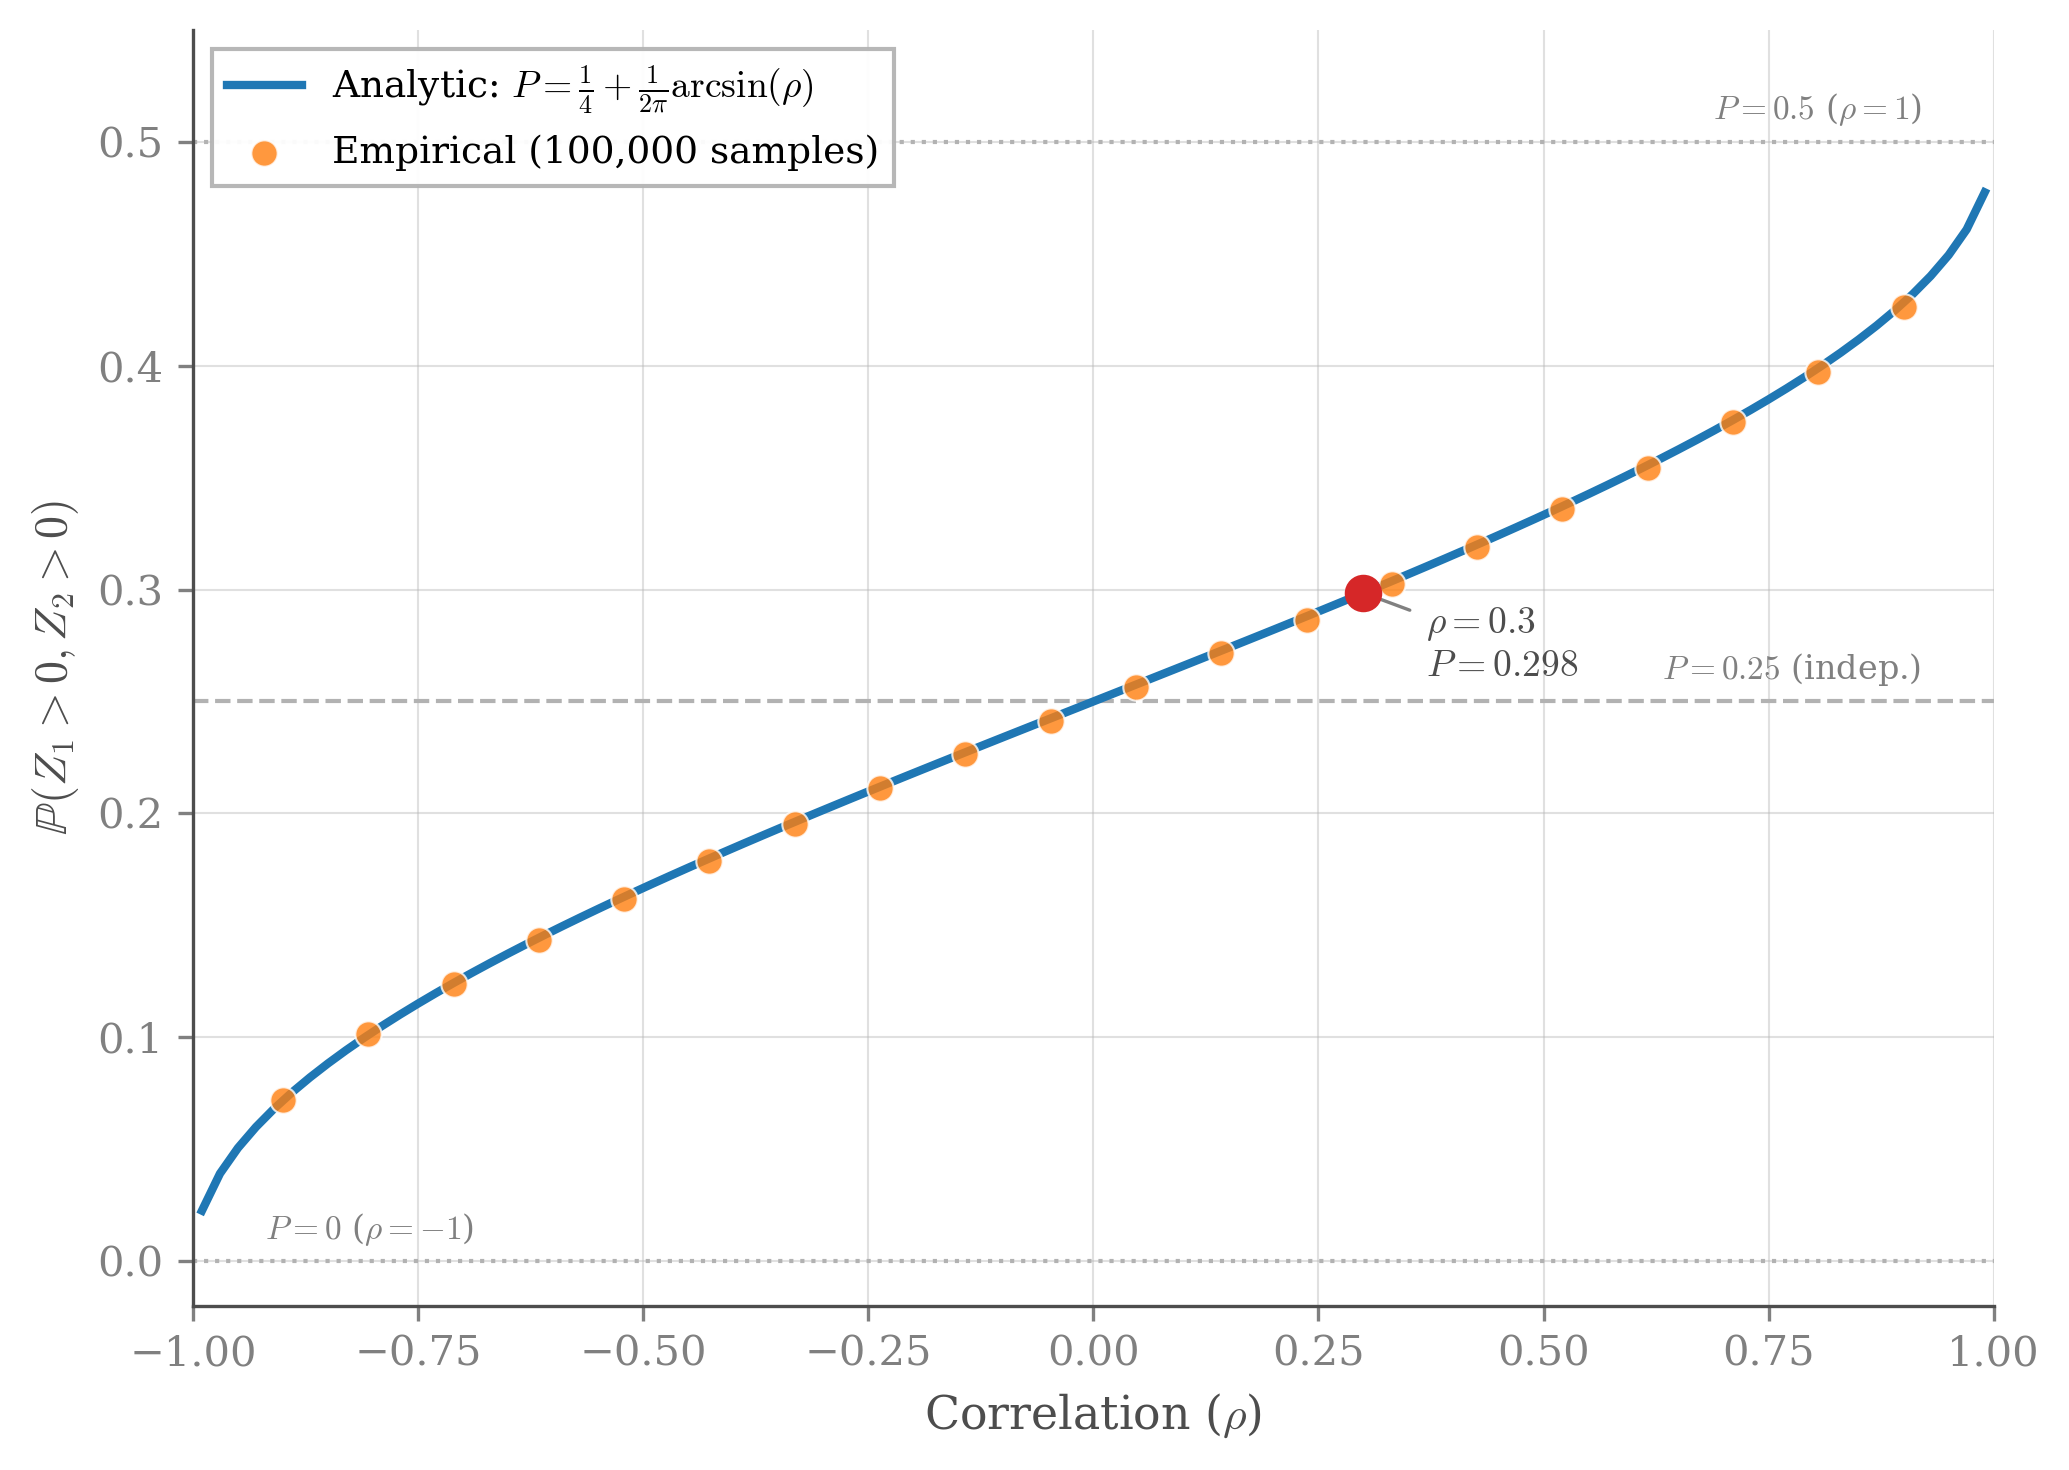
\includegraphics[width=0.9\linewidth]{../figures/joint_exceedance_vs_rho.png}
  \caption[Gaussian copula joint exceedance]{Gaussian-copula joint exceedance at symmetric thresholds ($z_1=z_2=0$) as a function of correlation $\rho$. The analytic curve $\Prob(Z_1>0,Z_2>0)=\tfrac14+\tfrac{1}{2\pi}\arcsin(\rho)$ provides a calibration check for dependence modeling (\Cref{subsec:copula-st}).}
  \label{fig:copula-joint}
\end{figure}

\subsection{Tail Refinements: Edgeworth and Saddlepoint Approximations}
\label{subsec:edgeworth}

Let $M$ be integer margin with mean $\mu_D$, variance $\sigma_D^2$, standardized $Z=(M-\mu_D)/\sigma_D$, skewness $\gamma_1$ and kurtosis $\gamma_2$. The Edgeworth approximation to $\Prob(M\le m)$ is
\[
\Phi(z)+\phi(z)\!\left(\frac{\gamma_1}{6}(z^2-1)+\frac{\gamma_2}{24}(z^3-3z)+\frac{\gamma_1^2}{72}(z^5-10z^3+15z)\right),
\]
$z=(m+\tfrac12-\mu_D)/\sigma_D$ (continuity-corrected). For lattice accuracy at extreme tails we also use the saddlepoint approximation with cumulant generator $K(t)=\log \E[e^{tM}]$:
\[
\Prob(M=m)\approx \frac{1}{\sqrt{2\pi K''(\hat t)}}\exp\!\big(K(\hat t)-\hat t\,m\big),
\quad \text{with }K'(\hat t)=m.
\]
Classical accuracy results for saddlepoint/Edgeworth approximations include \citet{daniels1954}; see also \Cref{subsec:crps-lattice} for discrete-evaluation implications.

%=============================================================================
% TIER 3: MACHINE LEARNING METHODS
%=============================================================================
\section{Machine Learning Methods}
\label{sec:ml-methods}

This section surveys the machine learning techniques that complement classical statistical models, with emphasis on gradient boosting, ensemble methods, and feature attribution.

\subsection{Gradient Boosting: XGBoost and LightGBM}
\label{subsec:gradient-boosting}

Gradient boosting \citep{friedman2001} constructs an additive model by sequentially fitting weak learners to pseudo-residuals of a differentiable loss function. For a loss $L(y, F(x))$ and current model $F_m$, the next learner $h_{m+1}$ approximates the negative gradient:
\begin{equation}
h_{m+1}(x) \approx -\left[\frac{\partial L(y, F(x))}{\partial F(x)}\right]_{F=F_m}.
\end{equation}
The model updates via $F_{m+1}(x) = F_m(x) + \nu h_{m+1}(x)$ with learning rate $\nu \in (0,1]$.

\paragraph{XGBoost.} \citet{chen2016xgboost} introduced regularized gradient boosting with several innovations: (i) a regularized objective $\mathcal{L}(\theta) = \sum_i l(y_i, \hat{y}_i) + \sum_k \Omega(f_k)$ where $\Omega(f) = \gamma T + \frac{1}{2}\lambda\|w\|^2$ penalizes tree complexity; (ii) second-order Taylor expansion of the loss for efficient split finding; (iii) sparsity-aware algorithms for missing values; and (iv) column subsampling inspired by random forests. The closed-form optimal leaf weight and split gain are:
\begin{align}
w_j^* &= -\frac{\sum_{i \in I_j} g_i}{\sum_{i \in I_j} h_i + \lambda}, \label{eq:xgb-leaf}\\
\mathcal{L}_{\text{split}} &= \frac{1}{2}\left[\frac{(\sum_{i \in I_L} g_i)^2}{\sum_{i \in I_L} h_i + \lambda} + \frac{(\sum_{i \in I_R} g_i)^2}{\sum_{i \in I_R} h_i + \lambda} - \frac{(\sum_{i \in I} g_i)^2}{\sum_{i \in I} h_i + \lambda}\right] - \gamma, \label{eq:xgb-gain}
\end{align}
where $g_i = \partial l / \partial \hat{y}_i$ and $h_i = \partial^2 l / \partial \hat{y}_i^2$ are first and second derivatives.

\paragraph{LightGBM.} \citet{ke2017lightgbm} further improved scalability via gradient-based one-side sampling (GOSS) and exclusive feature bundling (EFB), achieving 20$\times$ speedup on large datasets while maintaining accuracy. Leaf-wise (best-first) tree growth often produces deeper, more accurate trees than XGBoost's level-wise approach.

\paragraph{Hyperparameter sensitivity.} Key parameters include max depth (3--8), learning rate (0.01--0.3), L1/L2 regularization ($\alpha$, $\lambda$), and subsampling rates. \citet{probst2019tunability} demonstrate that boosting methods are among the most hyperparameter-sensitive, motivating careful cross-validation. For NFL prediction, shallow trees (depth 3--5) with strong regularization ($\lambda \geq 1.0$) help prevent overfitting to the limited sample size (~270 games/season).

\paragraph{Application to sports prediction.} Gradient boosting has become the dominant approach for tabular sports prediction due to its handling of heterogeneous features, automatic feature interaction discovery, and robustness to outliers. \citet{hubacek2019exploiting} demonstrate XGBoost's effectiveness for soccer prediction, while \citet{horvat2020impact} analyze its application to NBA outcomes. For NFL, the challenge is balancing model complexity against the small sample size; regularization and proper temporal validation are essential.

\subsection{Ensemble Methods: Theory and Practice}
\label{subsec:ensemble-theory}

Ensemble methods combine multiple models to reduce variance and improve robustness. We review three paradigms: model averaging, stacking, and negative correlation learning.

\subsubsection{Model Averaging and Variance Decomposition}

For an ensemble of $M$ models with predictions $\hat{f}_m$ and weights $w_m$ ($\sum w_m = 1$), the ensemble prediction is:
\begin{equation}
\hat{f}_{\text{ens}}(\mathbf{x}) = \sum_{m=1}^{M} w_m \hat{f}_m(\mathbf{x}).
\end{equation}
\citet{hansen1990neural} formalized the variance reduction principle. The mean squared error decomposes as:
\begin{equation}\label{eq:ensemble-decomposition}
\E\big[(\hat{f}_{\text{ens}} - y)^2\big] = \underbrace{\frac{1}{M} \bar{\sigma}^2}_{\text{Variance reduction}} + \underbrace{\left(1 - \frac{1}{M}\right) \bar{\rho} \bar{\sigma}^2}_{\text{Correlation penalty}} + \bar{B}^2,
\end{equation}
where $\bar{\sigma}^2 = \frac{1}{M}\sum_m \Var(\hat{f}_m)$ is mean component variance, $\bar{\rho}$ is average pairwise correlation, and $\bar{B}^2$ is mean squared bias.

\textbf{Key insight:} As $M \to \infty$ and $\bar{\rho} \to 0$, ensemble variance $\to 0$. When $\bar{\rho}$ is high (correlated models), variance reduction plateaus regardless of $M$. Therefore: \emph{adding uncorrelated weak models beats refining correlated strong models}. This motivates methodological diversity (Bayesian + frequentist + ML) over hyperparameter tuning within a single paradigm.

\subsubsection{Stacking and Meta-Learning}

\citet{wolpert1992stacked} introduced stacked generalization, where a meta-learner combines base model predictions. Given base predictions $\hat{f}_1(x), \ldots, \hat{f}_M(x)$, the stacked predictor is:
\begin{equation}
\hat{f}_{\text{stack}}(x) = g\big(\hat{f}_1(x), \ldots, \hat{f}_M(x); \theta\big),
\end{equation}
where $g$ is a meta-model (often linear or gradient boosting) trained on out-of-fold base predictions to avoid overfitting.

\citet{breiman1996stacked} showed that stacking with non-negative constrained linear regression achieves optimal asymptotic risk. \citet{yao2018stacking} extended this to Bayesian model averaging (BMA) and stacking under log-score, showing that stacking outperforms BMA when models are misspecified---the typical case in practice.

\paragraph{Bayesian Model Averaging vs.\ Stacking.} BMA weights models by posterior probability $p(M_k | D)$, which requires specifying prior model probabilities and can be dominated by a single model. Stacking optimizes predictive performance directly:
\begin{equation}
\hat{w} = \arg\min_{w \in \Delta^{M-1}} \sum_{i=1}^n L\left(y_i, \sum_{m=1}^M w_m \hat{f}_m^{(-i)}(x_i)\right),
\end{equation}
where $\hat{f}_m^{(-i)}$ is the $m$-th model's prediction trained without observation $i$. \citet{yao2018stacking} recommend stacking for prediction tasks where model misspecification is expected.

\subsubsection{Negative Correlation Learning}

\citet{liu1999ensemble} introduced negative correlation learning (NCL), which explicitly penalizes correlation during training:
\begin{equation}
L_m = \frac{1}{2}(f_m(x) - y)^2 + \lambda \cdot (f_m(x) - \bar{f}(x)) \cdot \sum_{j \neq m}(f_j(x) - \bar{f}(x)),
\end{equation}
where $\bar{f}(x) = \frac{1}{M}\sum_m f_m(x)$. The penalty term encourages diversity by pushing each model's prediction away from the ensemble mean when other models are also deviating.

\paragraph{Dirichlet Ensemble Weights.} For continuous weight optimization, a Dirichlet prior $w \sim \text{Dir}(\alpha)$ provides regularization toward uniform weights when $\alpha_m = \alpha_0$ for all $m$. Higher $\alpha_0$ increases regularization strength. The posterior mode under squared loss is:
\begin{equation}
\hat{w}_m \propto \frac{\alpha_m - 1 + \sum_i \hat{f}_m(x_i)(y_i - \bar{y})}{\sum_i \hat{f}_m(x_i)^2},
\end{equation}
subject to simplex constraints. This provides a principled approach to weight learning that avoids extreme weights while adapting to model performance.

\subsection{Feature Attribution: Shapley Values and SHAP}
\label{subsec:shapley}

Interpreting complex models requires principled attribution of predictions to input features. \citet{shapley1953value} introduced a game-theoretic solution concept with uniquely desirable properties.

\paragraph{Shapley values.} For a set function $v: 2^N \to \mathbb{R}$ (the ``game'') over $N$ players (features), the Shapley value for player $i$ is:
\begin{equation}\label{eq:shapley}
\phi_i(v) = \sum_{S \subseteq N \setminus \{i\}} \frac{|S|!(|N|-|S|-1)!}{|N|!} \big[v(S \cup \{i\}) - v(S)\big].
\end{equation}
This is the unique attribution satisfying: (i) efficiency ($\sum_i \phi_i = v(N) - v(\emptyset)$), (ii) symmetry (equal contribution $\Rightarrow$ equal attribution), (iii) linearity, and (iv) null player ($v(S \cup \{i\}) = v(S)$ for all $S$ $\Rightarrow$ $\phi_i = 0$).

\paragraph{SHAP.} \citet{lundberg2017unified} connected Shapley values to machine learning interpretation via SHAP (SHapley Additive exPlanations). For a model $f$ and input $x$, define:
\begin{equation}
v_x(S) = \E[f(X) | X_S = x_S],
\end{equation}
the expected prediction when features in $S$ are fixed to their values in $x$. The SHAP value $\phi_i(x) = \phi_i(v_x)$ then attributes the prediction $f(x) - \E[f(X)]$ to each feature.

\paragraph{TreeSHAP.} Computing exact Shapley values requires $O(2^N)$ subset evaluations. \citet{lundberg2020local} developed TreeSHAP, which computes exact SHAP values for tree ensembles in $O(TLD^2)$ time, where $T$ is number of trees, $L$ is maximum leaves, and $D$ is maximum depth. This enables practical interpretation of gradient boosting models.

\paragraph{SHAP interactions.} For pairwise feature interactions, the Shapley interaction index \citep{grabisch1999axiomatic} extends to:
\begin{equation}
\Phi_{ij} = \sum_{S \subseteq N \setminus \{i,j\}} \frac{|S|!(|N|-|S|-2)!}{2(|N|-1)!} \Delta_{ij}(S),
\end{equation}
where $\Delta_{ij}(S) = v(S \cup \{i,j\}) - v(S \cup \{i\}) - v(S \cup \{j\}) + v(S)$. This quantifies synergistic or redundant effects between features.

\paragraph{Application to sports analytics.} SHAP values enable understanding which features drive individual predictions (local interpretation) and which are globally important (mean absolute SHAP). For betting, this supports: (i) identifying when a model relies on unstable features, (ii) detecting potential data leakage through implausibly high attributions, and (iii) explaining predictions to stakeholders.

\subsection{Conformal Prediction}
\label{subsec:conformal}

Conformal prediction \citep{vovk2005algorithmic} provides distribution-free prediction intervals with finite-sample coverage guarantees. Unlike asymptotic confidence intervals, conformal methods are valid for any sample size under exchangeability.

\paragraph{Split conformal prediction.} Given a calibration set $\{(X_i, Y_i)\}_{i=1}^n$ and a trained model $\hat{f}$, define nonconformity scores $s_i = |Y_i - \hat{f}(X_i)|$ (for regression). The $(1-\alpha)$ prediction interval for a new point $X_{n+1}$ is:
\begin{equation}\label{eq:conformal-interval-lit}
\hat{C}(X_{n+1}) = \left[\hat{f}(X_{n+1}) - \hat{q}, \hat{f}(X_{n+1}) + \hat{q}\right],
\end{equation}
where $\hat{q}$ is the $\lceil(n+1)(1-\alpha)\rceil/n$ quantile of the calibration scores. This guarantees:
\begin{equation}
\Pr(Y_{n+1} \in \hat{C}(X_{n+1})) \geq 1 - \alpha,
\end{equation}
for exchangeable $(X_1, Y_1), \ldots, (X_{n+1}, Y_{n+1})$.

\paragraph{Conformalized quantile regression.} \citet{romano2019conformalized} showed that using quantile regression residuals as nonconformity scores produces adaptive intervals---narrower when the model is confident, wider when uncertain:
\begin{equation}
s_i = \max\left\{\hat{q}_{\alpha/2}(X_i) - Y_i, Y_i - \hat{q}_{1-\alpha/2}(X_i)\right\}.
\end{equation}

\paragraph{Weighted conformal prediction.} Standard conformal prediction requires exchangeability, which fails under covariate shift or temporal dependence. \citet{tibshirani2019conformal} introduced weighted conformal prediction:
\begin{equation}
\hat{q}_w = \inf\left\{q : \sum_{i=1}^n w_i \mathbb{1}\{s_i \leq q\} \geq (1-\alpha)\sum_{i=1}^n w_i\right\},
\end{equation}
where weights $w_i$ downweight observations dissimilar to the test point. For temporal data, exponential decay weights $w_i = \exp(-\lambda(n-i))$ address non-stationarity while preserving approximate coverage.

\paragraph{Application to sports betting.} Conformal intervals provide calibrated uncertainty without distributional assumptions. For betting, wide intervals signal unreliable predictions where stakes should be reduced. The coverage guarantee holds even when the underlying model is misspecified, providing a safety layer for the decision system.

\subsection{Online Learning and Concept Drift}
\label{subsec:online-learning}

Sports data exhibit non-stationarity due to rule changes, strategic evolution, and roster turnover. Online learning methods adapt to such \emph{concept drift} without full retraining.

\paragraph{Types of drift.} \citet{gama2014survey} categorize drift as: (i) \emph{sudden} (abrupt change, e.g., major rule modification), (ii) \emph{gradual} (slow transition between concepts), (iii) \emph{incremental} (continuous evolution), and (iv) \emph{recurring} (periodic patterns, e.g., seasonal effects). NFL prediction faces all types: rule changes cause sudden drift, strategic meta-game evolution is gradual, and early-season uncertainty recurs annually.

\paragraph{Drift detection.} The Page-Hinkley test \citep{page1954continuous} monitors cumulative deviation from a baseline:
\begin{equation}
m_t = \sum_{i=1}^t (x_i - \bar{x}_t - \delta), \quad M_t = \max_{1 \leq j \leq t} m_j,
\end{equation}
where drift is signaled when $M_t - m_t > \lambda$. ADWIN \citep{bifet2007learning} automatically adjusts window size, shrinking when drift is detected and growing during stable periods.

\paragraph{Adaptive ensembles.} Rather than detecting and reacting to drift, adaptive ensembles continuously adjust. \citet{kolter2007dynamic} propose Dynamic Weighted Majority, which maintains a pool of experts and adjusts weights based on recent performance:
\begin{equation}
w_m^{(t+1)} = w_m^{(t)} \cdot \beta^{\mathbb{1}\{\hat{y}_m^{(t)} \neq y^{(t)}\}},
\end{equation}
where $\beta \in (0,1)$ is a decay factor. Poorly performing experts are removed and new experts added periodically.

\paragraph{Online gradient descent.} For differentiable losses, online gradient descent \citep{zinkevich2003online} updates parameters after each observation:
\begin{equation}
\theta^{(t+1)} = \theta^{(t)} - \eta_t \nabla L(y^{(t)}, f(x^{(t)}; \theta^{(t)})).
\end{equation}
With appropriate learning rate schedules ($\eta_t = O(1/\sqrt{t})$), regret bounds guarantee near-optimal performance relative to the best fixed predictor in hindsight.

\paragraph{Application to NFL prediction.} Weekly model updates using online learning can capture within-season drift (injuries, form changes) without overfitting to noise. Exponentially weighted moving averages of feature distributions support drift detection, triggering recalibration when distributions shift significantly from training.

%=============================================================================
% TIER 4: EVALUATION AND CALIBRATION
%=============================================================================
\section{Evaluation and Calibration}
\label{sec:evaluation}

Reliable predictions require both accuracy and calibration. This section covers proper scoring rules, reliability assessment, and uncertainty quantification methods.

\subsection{Proper Scoring Rules}
\label{subsec:proper-scoring}

\citet{gneiting2007strictly} provide a comprehensive treatment of scoring rules for probabilistic forecasts. A scoring rule $S(P, y)$ assigns a numerical score to a probabilistic forecast $P$ when outcome $y$ is observed.

\paragraph{Strictly proper scores.} A scoring rule is \emph{strictly proper} if the expected score is uniquely maximized when the forecast equals the true distribution: $\E_{Y \sim Q}[S(P, Y)]$ is maximized iff $P = Q$. Key examples include:

\begin{itemize}
  \item \textbf{Log score (negative log-loss):} $S(P, y) = \log P(y)$
  \item \textbf{Brier score:} For binary outcomes, $S(p, y) = -(p - y)^2$
  \item \textbf{Continuous Ranked Probability Score (CRPS):} For distributions,
  \begin{equation}\label{eq:crps}
  \mathrm{CRPS}(F, y) = -\int_{-\infty}^{\infty} \big(F(z) - \mathbb{1}\{z \geq y\}\big)^2 \, dz.
  \end{equation}
\end{itemize}

\paragraph{Brier score decomposition.} The Brier score admits a useful decomposition \citep{murphy1973new}:
\begin{equation}
\text{BS} = \underbrace{\frac{1}{n}\sum_{k=1}^K n_k(\bar{p}_k - \bar{y}_k)^2}_{\text{Reliability}} - \underbrace{\frac{1}{n}\sum_{k=1}^K n_k(\bar{y}_k - \bar{y})^2}_{\text{Resolution}} + \underbrace{\bar{y}(1-\bar{y})}_{\text{Uncertainty}},
\end{equation}
where forecasts are binned by predicted probability, $\bar{p}_k$ is the mean prediction in bin $k$, $\bar{y}_k$ is the empirical frequency, and $\bar{y}$ is the overall base rate. Reliability measures calibration (smaller is better); resolution measures ability to discriminate (larger is better).

\paragraph{CRPS on lattices.}\label{subsec:crps-lattice}
For integer margins we work with a lattice distribution $F$ on $\mathbb{Z}$. The CRPS can be written as
\begin{equation}
\mathrm{CRPS}(F,y)=\sum_{m\in\mathbb Z} \big(F(m)-\mathbb 1\{m\ge y\}\big)^2\,\Delta_m,\qquad \Delta_m=1,
\end{equation}
which is the discrete analogue of the $L^2$ distance between $F$ and the step function at $y$. Taking expectation w.r.t.\ the true $Y\sim F^\star$ yields $\mathbb E\,\mathrm{CRPS}(F,Y)= \|F-F^\star\|_{L^2}^2 + \text{const}$, since $\mathbb E\,\mathbb 1\{m\ge Y\}=1-F^\star(m-1)$. Hence the unique minimizer is $F=F^\star$, showing strict propriety on the lattice.

\subsection{Reliability Diagrams and Expected Calibration Error}
\label{subsec:reliability}

Reliability diagrams visualize calibration by plotting empirical frequencies against predicted probabilities. For predictions binned into $K$ intervals, plot $(\bar{p}_k, \bar{y}_k)$ for each bin; perfect calibration lies on the diagonal.

\paragraph{Expected Calibration Error.} The ECE summarizes miscalibration:
\begin{equation}
\text{ECE} = \sum_{k=1}^K \frac{n_k}{n} |\bar{p}_k - \bar{y}_k|.
\end{equation}
\citet{naeini2015obtaining} recommend equal-frequency bins to avoid empty or sparse bins. For small samples, bootstrap confidence bands quantify uncertainty in the reliability diagram.

\paragraph{Calibration methods.} When models are miscalibrated, post-hoc calibration can help:
\begin{itemize}
  \item \textbf{Platt scaling} \citep{platt1999probabilistic}: Fit logistic regression $\sigma(a \cdot f(x) + b)$ on held-out predictions.
  \item \textbf{Isotonic regression}: Non-parametric monotonic mapping from predictions to calibrated probabilities.
  \item \textbf{Temperature scaling} \citep{guo2017calibration}: For multi-class, divide logits by temperature $T$ before softmax.
\end{itemize}

% Reliability diagram with binomial confidence intervals
\begin{figure}[t]
  \centering
  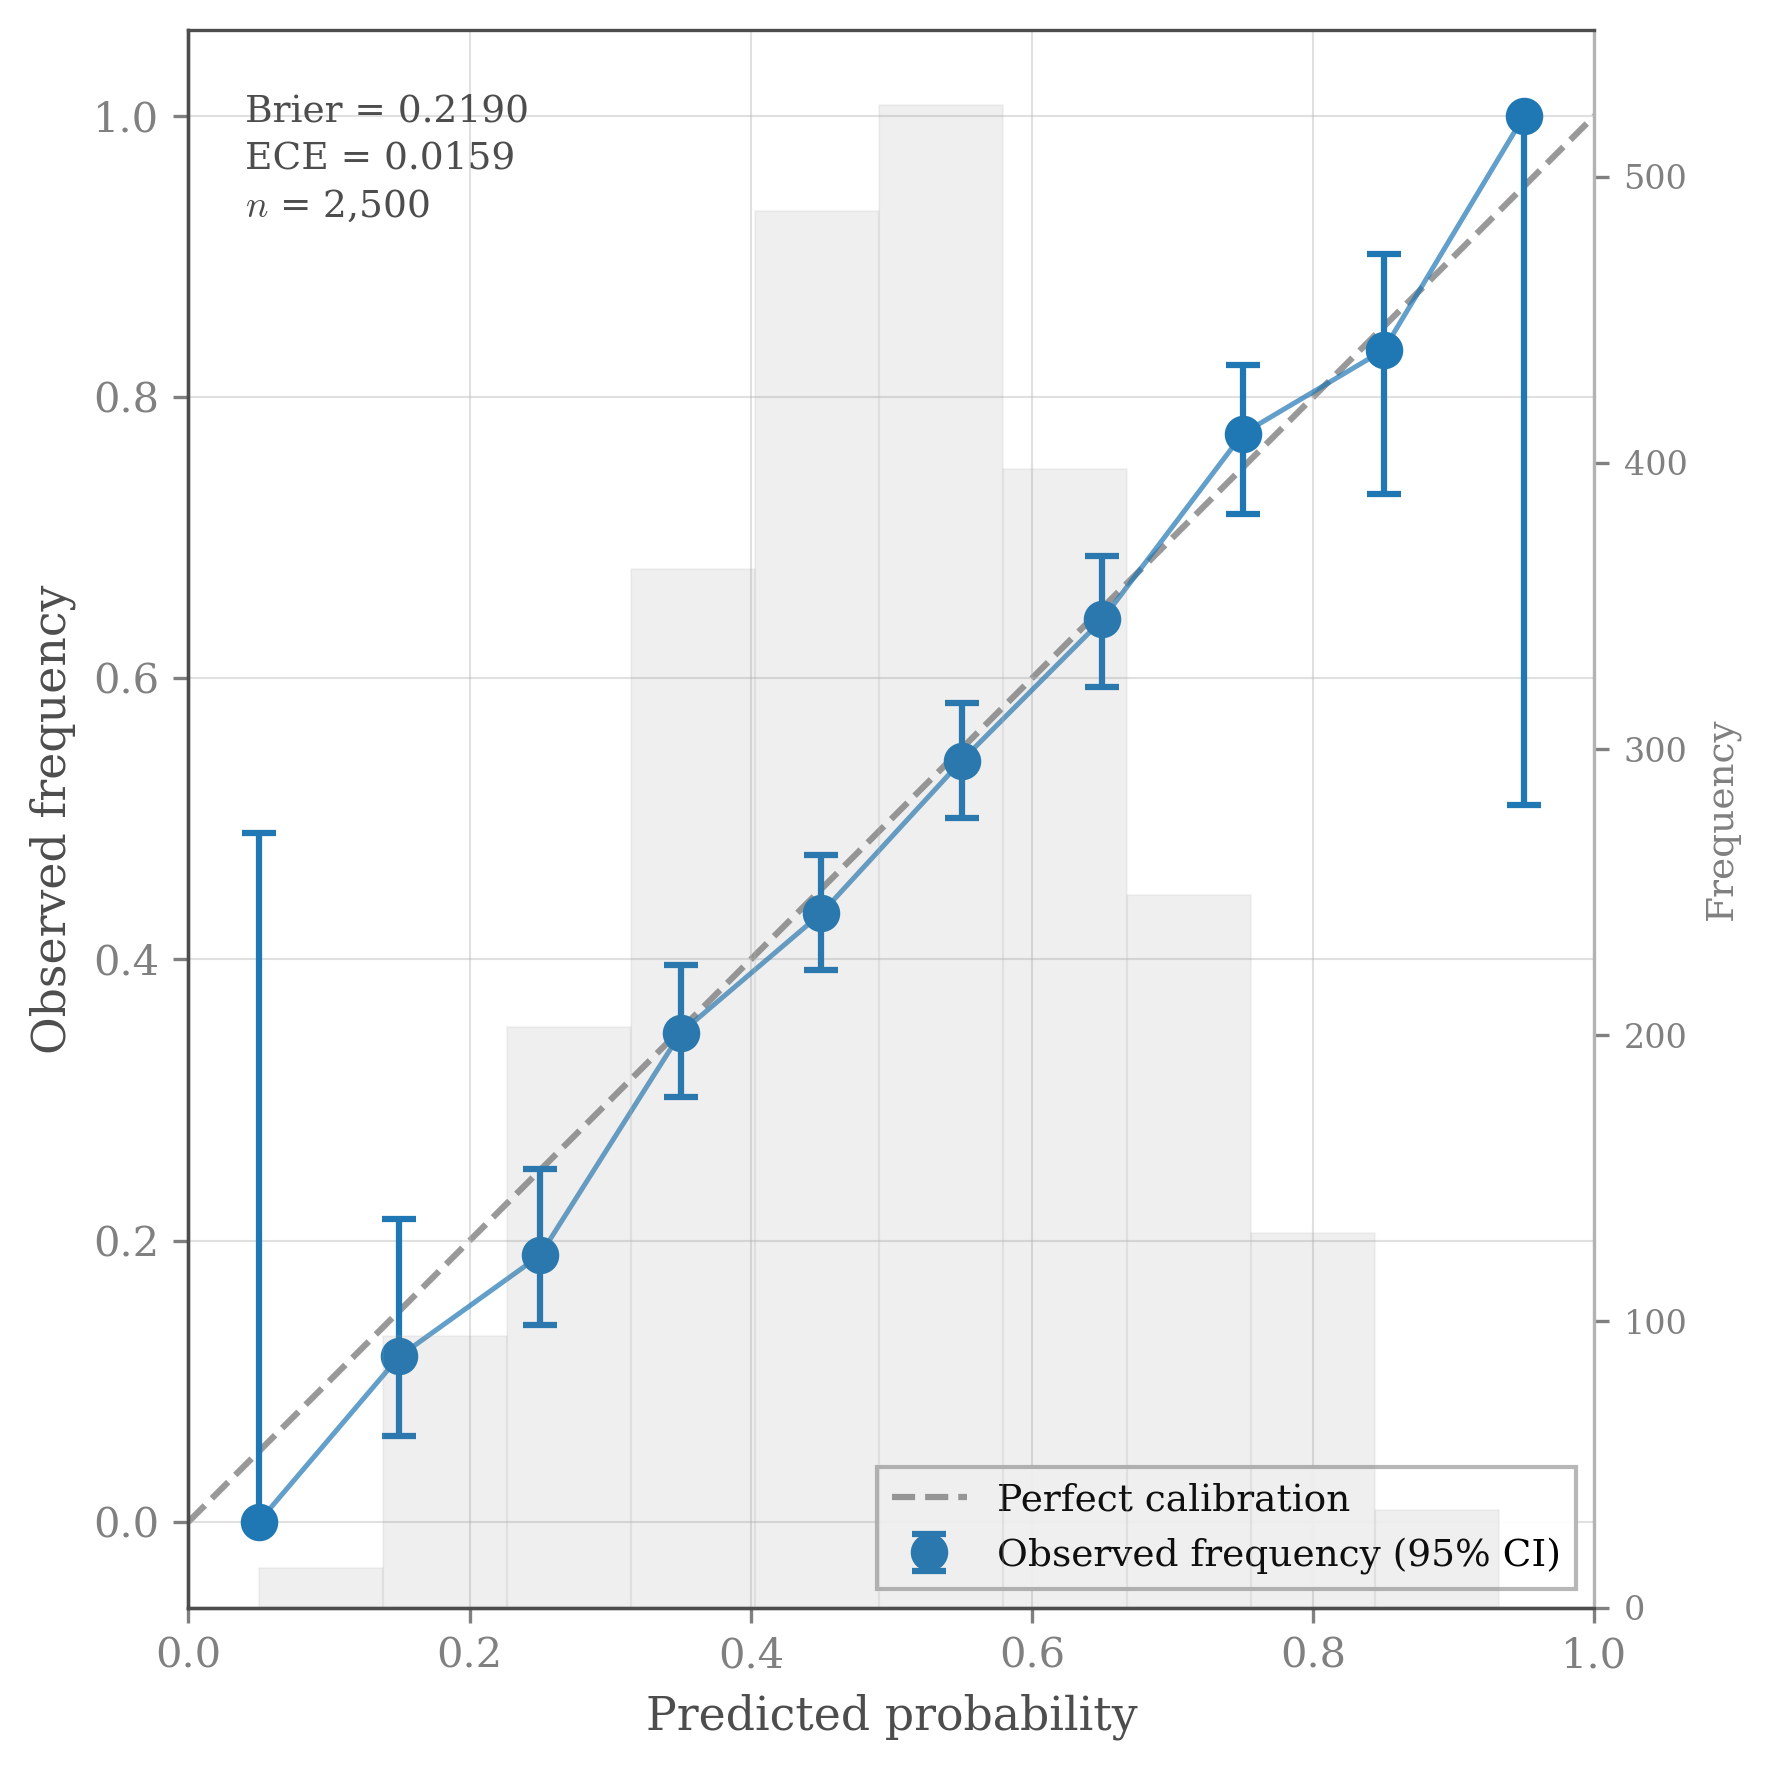
\includegraphics[width=0.9\linewidth]{../figures/reliability_diagram.png}
  \caption[Reliability diagram (95\% CIs)]{Reliability diagram with 95\% binomial confidence intervals. Points show empirical frequencies by predicted-probability bin; the diagonal indicates perfect calibration. We report these alongside Brier/log-loss and ECE.}
  \label{fig:reliability}
\end{figure}

\subsection{Uncertainty Quantification Methods}
\label{subsec:uq-methods}

Beyond point predictions, quantifying uncertainty enables risk-aware decision-making. We survey five approaches:

\paragraph{Bayesian posteriors.} Bayesian models provide posterior predictive distributions by construction. For state-space models (\Cref{subsec:glickman1998}), the Kalman filter yields Gaussian posteriors; for hierarchical models, MCMC samples approximate the posterior.

\paragraph{Bootstrap.} Resampling training data produces an ensemble of models whose prediction variance estimates uncertainty \citep{efron1994introduction}. For structured data (games within seasons), block bootstrap preserves temporal dependence.

\paragraph{Quantile regression.} Direct estimation of conditional quantiles $Q_\tau(Y|X)$ for $\tau \in (0,1)$ provides prediction intervals without distributional assumptions \citep{koenker2005quantile}. Gradient boosting with pinball loss enables flexible quantile estimation.

\paragraph{MC Dropout.} \citet{gal2016dropout} showed that dropout at test time approximates Bayesian inference. Predictions with $T$ forward passes yield mean and variance:
\begin{equation}
\hat{y} = \frac{1}{T}\sum_{t=1}^T f_{\theta_t}(x), \quad \hat{\sigma}^2 = \frac{1}{T}\sum_{t=1}^T f_{\theta_t}(x)^2 - \hat{y}^2,
\end{equation}
where $\theta_t$ represents the $t$-th dropout mask.

\paragraph{Evidential regression.} \citet{amini2020deep} proposed learning a distribution over distributions---specifically, a Normal-Inverse-Gamma prior for regression. The network outputs $(\gamma, \nu, \alpha, \beta)$ parameterizing $\text{NIG}(\gamma, \nu, \alpha, \beta)$, from which epistemic and aleatoric uncertainty are derived. This provides uncertainty in a single forward pass, trading accuracy for speed.

\subsection{Evaluation Protocols and Temporal Validation}
\label{subsec:temporal-validation}

Sports prediction requires temporal cross-validation to prevent future information leakage.

\paragraph{Rolling origin.} Train on seasons $1, \ldots, t-1$; validate on season $t$; increment $t$. This simulates realistic deployment where only past data is available.

\paragraph{Blocked time series.} Within seasons, block by week: train on weeks $1, \ldots, w-1$; predict week $w$; update. This tests within-season adaptation.

\paragraph{Leakage prevention.} Strict temporal ordering prevents: (i) using closing lines before game time, (ii) incorporating injury updates announced after line release, (iii) training on seasons after the validation period. Feature engineering pipelines must respect ``as-of'' timestamps.

%=============================================================================
% TIER 5: DECISION THEORY
%=============================================================================
\section{Decision Theory for Sports Betting}
\label{sec:decision-theory}

Predictions gain value only through optimal decisions. This section connects probabilistic forecasts to wagering strategies via Kelly criterion, game-theoretic framing, and market microstructure.

\subsection{Kelly Criterion and Optimal Betting}
\label{subsec:kelly}

\citet{kelly1956new} derived the stake fraction maximizing expected log-wealth growth. For a binary bet with win probability $p$ and decimal odds $d$:
\begin{equation}\label{eq:kelly}
f^* = \frac{p \cdot d - 1}{d - 1} = \frac{p - q/d}{1 - 1/d},
\end{equation}
where $q = 1-p$. This is positive iff $p > 1/d$ (positive expected value).

\paragraph{Properties.} Kelly betting maximizes the long-run geometric growth rate $G = \E[\log(1 + f \cdot R)]$ where $R \in \{d-1, -1\}$. It asymptotically dominates any essentially different strategy but exhibits high variance, motivating fractional Kelly ($\lambda f^*$ with $\lambda < 1$).

\paragraph{Kelly with uncertainty.} When $p$ is estimated with uncertainty, replacing $p$ by a lower confidence bound yields a risk-aware variant:
\begin{equation}
f_{\text{LCB}} = \max\left\{0, \frac{(p - k\sigma_p) \cdot d - 1}{d - 1}\right\},
\end{equation}
where $\sigma_p$ is the standard error of $\hat{p}$ and $k$ controls conservatism. This connects to the CVaR-constrained staking developed in \Cref{chap:risk}.

\subsection{Vigorish Removal and Comparative Book Value}
\label{subsec:vig-cbv}

For a two-outcome market with American odds $(o_1, o_2)$, convert to decimals $(d_1, d_2)$ and implied probabilities $\pi_i^{\mathrm{raw}} = 1/d_i$. The hold (vig) is $H = \pi_1^{\mathrm{raw}} + \pi_2^{\mathrm{raw}} - 1$. No-vig probabilities are $\pi_i = \pi_i^{\mathrm{raw}}/(1+H)$.

Given model fair probability $\hat{\pi}_i$, the \emph{Comparative Book Value} is:
\begin{equation}
\mathrm{CBV}_i = \hat{\pi}_i - \pi_i,
\end{equation}
or in price space $\Delta_i = d_i - (1/\hat{\pi}_i)$. Positive CBV indicates the model assigns higher probability than the market implies. We bet when $\mathrm{CBV}_i > \tau$ for threshold $\tau$ that accounts for estimation error and transaction costs.

\subsection{Game-Theoretic Foundations}
\label{subsec:game-theory}

Bookmakers and bettors form a strategic ecosystem with asymmetric information, inventory constraints, and repeated interaction.

\paragraph{Risk-aware market maker.} Let $\pi$ be prices (implied probs) and $Q(\pi)$ the net demand vector. With outcome randomness $\theta$, one stylized objective is:
\begin{equation}
\max_{\pi}\; \E_\theta[\Pi(\pi;\theta)] - \lambda\,\Var_\theta[\Pi(\pi;\theta)] - \gamma\,\|Q(\pi)\|_2^2,
\end{equation}
where $\lambda, \gamma \geq 0$ encode risk and inventory costs. First-order conditions imply \emph{price shading} against imbalanced flow, increasing with outcome variance and demand inelasticity.

\paragraph{Implications for prediction.} Game-theoretic frictions predict pockets of inefficiency where: (i) inventory/rounding bites (key numbers), (ii) information latency is high (late injury/weather), or (iii) demand is biased (favorites/popular teams). Our ablations target exactly these loci.

\subsection{Market Microstructure}
\label{subsec:microstructure}

\paragraph{Economics of wagering markets.} \citet{sauer1998economics} surveys the structure and efficiency of wagering markets, including bookmaker margins, bettor behavior models, and informational asymmetries. \citet{levitt2004sports} argues bookmakers sometimes exploit bettor biases (e.g., overbetting favorites) rather than purely balancing books.

\paragraph{Closing-line efficiency.} The closing line aggregates information efficiently on average, serving as a benchmark for model performance. \citet{kaunitz2017beating} demonstrated that even small, consistent outperformance of closing lines yields positive returns, though limits and account restrictions present practical challenges.

\paragraph{Cross-market dependence.} Spreads, totals, and moneylines share latent factors (team strength, tempo). Correlation structures induced by shared information affect correlated parlays and same-game parlays, motivating the copula-based dependence modeling in \Cref{subsec:copula-st}.

\paragraph{Market as signal.} We treat the market (closing lines) as both:
\begin{itemize}
  \item A performance benchmark: models must capture closing-line value (CLV) edge
  \item A feature: cross-book spreads, line velocity, implied vs model delta
\end{itemize}

\subsection{Mapping Predictions to Decision Value}
\label{subsec:prediction-to-value}

We connect statistical metrics to economic outcomes by writing expected value (EV) explicitly in terms of probabilities.

Consider a binary wager with decimal odds $d$ and true success probability $p$. The EV per unit stake is $\mathrm{EV}(p;d) = p \cdot d - 1$. If the book is no-vig with implied $\pi = 1/d$, then $\mathrm{EV}(p;\pi) = p/\pi - 1$. With a model probability $\hat{p} = p + \varepsilon$, the EV we act on is:
\begin{equation}
\mathrm{EV}(\hat{p};\pi) = \frac{\hat{p}}{\pi} - 1 = \frac{p}{\pi} - 1 + \frac{\varepsilon}{\pi}.
\end{equation}
Hence, conditional on placing the bet, the first-order EV error is $\varepsilon/\pi$. Averaging over bets, the mean absolute EV shortfall is controlled by the RMSE of $\varepsilon$; in particular, the Brier score $\E[\varepsilon^2]$ upper-bounds the average EV loss up to scale factor $1/\pi^2$.

Selection adds a gating effect: trades are taken only when $\hat{p} \geq \pi + \tau_\pi$. Near the threshold, false positives/negatives occur with probability proportional to the density of $\hat{p}$ at $\pi$, and their EV impact scales with $\partial\,\mathrm{EV}/\partial p|_{p=\pi} = 1/\pi$. Thus reducing calibration error (Brier/RMSE) and sharpening uncertainty jointly improves realized EV.

%=============================================================================
% TIER 6: EMERGING METHODS
%=============================================================================
\section{Emerging Methods}
\label{sec:emerging}

This section surveys recent advances from deep learning, causal inference, and production machine learning that inform future extensions.

\subsection{Sequence Models and Attention Mechanisms}
\label{subsec:transformers}

Transformer architectures \citep{vaswani2017attention} have revolutionized sequence modeling, with recent applications to time series forecasting.

\paragraph{Informer.} \citet{zhou2021informer} introduce ProbSparse self-attention, reducing $O(n^2)$ complexity to $O(n \log n)$, enabling efficient long-sequence forecasting. This is relevant for NFL prediction where team performance trajectories span 17-week seasons with complex temporal dependencies.

\paragraph{Temporal Fusion Transformer.} \citet{lim2021temporal} combine multi-horizon forecasting with interpretable attention mechanisms. The variable selection network identifies which static (team identity, stadium) and dynamic (injuries, form) features matter at each prediction horizon.

\paragraph{Hybrid attention-state-space models.} The Autoformer \citep{wu2021autoformer} decomposes series into trend and seasonal components before applying attention. For NFL applications, this could capture the interaction between team strength evolution (state-space) and game-specific contextual factors (attention).

\paragraph{Implications.} While current state-space models assume Markov dynamics, attention mechanisms could relax this assumption, allowing long-range dependencies (e.g., performance against specific opponent types) to inform predictions. Transformer-based extensions represent a primary research vector for future work.

\subsection{Causal Inference in Sports Analytics}
\label{subsec:causal}

Sports prediction typically focuses on association rather than causation. The distinction becomes critical when evaluating interventions, adjusting for confounders, and avoiding spurious correlations.

\paragraph{Potential outcomes framework.} \citet{imbens2015causal} define causal effects as contrasts between outcomes under different treatment assignments. The effect of a coaching change on win probability compares $Y^{(1)}$ (wins under new coach) with $Y^{(0)}$ (wins had old coach remained). The fundamental problem---observing only one potential outcome per unit---motivates matching, propensity weighting, and instrumental variable approaches.

\paragraph{DAG framework.} \citet{pearl2009causality} represent causal assumptions graphically with directed acyclic graphs. DAGs identify confounders requiring adjustment, mediators that should not be adjusted, and colliders that introduce spurious associations when conditioned upon. For NFL prediction, adjusting for opponent strength (a confounder of QB performance $\to$ game outcome) is essential, while adjusting for garbage-time stats (a mediator) would bias skill estimates.

\paragraph{Methods for sports.} Instrumental variables exploit exogenous variation: weather affects passing efficiency causally but is unrelated to team quality. \citet{hernan2020causal} provide accessible treatment of causal inference methods applicable to sports. Recent work by \citet{wang2024causal} connects causal inference to deep learning.

\paragraph{Implications.} Our Ridge Residuals methodology can be viewed through a causal lens: two-stage regression removes confounding by opponent quality, isolating ``pure skill.'' DAG-based feature selection could systematically identify which variables to include versus exclude.

\subsection{Large Language Models in Sports Analytics}
\label{subsec:llm}

Large Language Models (LLMs) offer potential for processing unstructured text, extracting entities, and performing complex reasoning about sports.

\paragraph{Sports-specific benchmarks.} \citet{xia2024sports} survey language and multimodal models in sports, cataloging datasets across multiple sports and task types. Domain-specific fine-tuning significantly improves tasks requiring temporal reasoning or statistical interpretation.

\paragraph{Retrieval-augmented generation.} RAG \citep{lewis2020retrieval} combines LLM reasoning with external knowledge retrieval, addressing hallucination risks. For NFL applications, RAG architectures could integrate play-by-play databases, injury reports, and news articles for sentiment signals.

\paragraph{Sentiment and entity extraction.} LLMs excel at Named Entity Recognition for injury reports (``Patrick Mahomes [PLAYER] is questionable [STATUS] with ankle [BODY\_PART]'') and sentiment analysis of media coverage. These capabilities inform semantic feature engineering.

\paragraph{Hallucination risks.} LLMs may generate plausible but incorrect information, particularly for recent events. Mitigation requires grounded retrieval and validation for high-stakes decisions.

\subsection{Production Machine Learning Systems}
\label{subsec:mlops}

Deploying ML models introduces challenges beyond accuracy: reproducibility, monitoring, versioning, and governance.

\paragraph{MLOps frameworks.} \citet{lwakatare2025mlops} propose maturity levels from ad-hoc experimentation through automated pipelines. Key components include data versioning, model registry, performance dashboards, and audit trails.

\paragraph{Model monitoring and drift detection.} Production models degrade under data drift (input distributions shift) or concept drift (input-output relationships change). For NFL prediction, drift sources include rule changes, strategic evolution, and roster turnover. Detection methods include statistical tests on feature distributions and performance monitoring by week.

\paragraph{Relevance.} Production architecture should implement containerized pipelines, model registries, and multi-season validation gates. Drift detection with automated monitoring enables timely recalibration.

%=============================================================================
% SYNTHESIS
%=============================================================================
\section{Synthesis and Research Gaps}
\label{sec:synthesis}

\subsection{Design Principles}

From the literature, our design principles are:
\begin{enumerate}
  \item Use Bayesian/shrinkage models to generate priors and uncertainty bounds.
  \item Use discrete margin/score distributions (bivariate Poisson + reweight) to price spreads, totals, teasers.
  \item Use ML meta-models to absorb nonlinear interactions among features.
  \item Employ rigorous calibration and proper scoring for model selection.
  \item Use decision theory (Kelly, CVaR) to convert edges into action sequences under risk constraints.
  \item Leverage the market as both a signal and benchmark; bet only when CBV passes threshold.
\end{enumerate}

\subsection{Classical vs.\ Modern: A Comparative Synthesis}

Classical models provide structure, interpretability, and tractable uncertainty, while modern ML models absorb nonlinear interactions and idiosyncrasies that generative assumptions miss. The hybrid approach leverages classical models for priors and calibration discipline, layering ML for residual structure and using decision theory to translate edges into actions under explicit constraints. This division of labor prevents ML from overfitting low-signal regimes and keeps decision-making grounded in uncertainty.

\paragraph{When classical wins.} In data-scarce or rapidly shifting regimes (e.g., early season, injury turbulence), shrinkage and state-space models dominate due to better calibrated uncertainty and temporal smoothing. Their transparent parameters support operational overrides.

\paragraph{When ML wins.} With stable covariates and rich features (market microstructure, team-form interactions), ML ensembles produce sharper probabilities. Calibration layers (Platt, isotonic) restore reliability while preserving sharpness.

\paragraph{Bridging to decision value.} Sharpness without calibration harms staking; calibration without sharpness limits EV. We therefore co-optimize for proper scoring rules and enforce economic gates (CBV thresholds, variance caps) to realize value.

\subsection{Research Gaps}

\Cref{tab:literature-gaps} identifies four key gaps in the uncertainty quantification literature that this dissertation addresses:

\begin{enumerate}
  \item \textbf{Temporal distribution shift:} Most UQ methods assume i.i.d.\ data, which sports data violate.
  \item \textbf{Single-method focus:} Prior work evaluates models in isolation; no cross-method comparison on identical test sets.
  \item \textbf{Speed-accuracy trade-off:} Academic papers optimize predictive metrics without considering inference latency.
  \item \textbf{Sports betting application:} UQ research focuses on safety-critical domains; sports betting is underrepresented.
\end{enumerate}

% Include the UQ methods comparison table
% !TEX root = ../main/main.tex
% uq_methods_comparison.tex
% Comprehensive comparison of 6 UQ methods across 6 dimensions
% Created: November 9, 2025

\begin{table}[p]
  \centering
  \caption[Uncertainty quantification methods comparison]{Uncertainty quantification methods: comprehensive comparison across six dimensions. Methods are ranked by computational cost (MCMC slowest, evidential fastest) and evaluated on coverage guarantees, assumptions, interpretability, and suitability for temporal drift.}
  \label{tab:uq-comparison}
  \begin{threeparttable}
  \small
  \setlength{\tabcolsep}{3pt}
  \renewcommand{\arraystretch}{1.25}
  \begin{tabularx}{\linewidth}{@{} l X X X X X @{}}
    \toprule
    \textbf{Method} & \textbf{Coverage Guarantee} & \textbf{Assumptions} & \textbf{Computation} & \textbf{Interpretability} & \textbf{Temporal Drift} \\
    \midrule

    \textbf{Bayesian MCMC}
    & Exact posterior (asymptotic); credible intervals calibrated if model correct
    & Parametric likelihood + prior; stationarity
    & $\mathcal{O}(IT \cdot n^3)$\tnote{a} per chain; 10--60s
    & High: priors, shrinkage, parameter interpretability
    & Poor: requires full retraining on drift; no online updates \\

    \midrule

    \textbf{MC Dropout}
    & Approximate Bayesian (variational); empirical calibration via sampling
    & Dropout $\approx$ Gaussian process prior; i.i.d.\ data
    & $\mathcal{O}(T \cdot \text{forward})$; 50--100 samples; 200--500ms
    & Low: black-box NN; dropout rate tuning unclear
    & Fair: incremental updates via SGD; prone to catastrophic forgetting \\

    \midrule

    \textbf{Conformal (CQR)}
    & Finite-sample coverage $\ge 1-\alpha$ (distribution-free)
    & Exchangeability (or weighted for covariate shift)
    & $\mathcal{O}(m \log m)$\tnote{b} calibration; <1ms per prediction
    & Medium: post-hoc correction; base model agnostic
    & Excellent: weighted conformal adapts to drift via time decay \\

    \midrule

    \textbf{Bayesian Stacking}
    & Ensemble coverage; empirical validation on LOO-CV
    & M-open (no model is "true"); proper scoring rule
    & $\mathcal{O}(K \cdot \text{model})$ + QP for weights\tnote{c}; 2--10s
    & Medium: interpretable weights; model-specific priors
    & Good: weight recomputation on new data; no full refit \\

    \midrule

    \textbf{Online Learning}
    & Asymptotic (PAC-style bounds); empirical coverage monitored
    & Incremental updates; drift detection (ADWIN)
    & $\mathcal{O}(1)$ per sample; $\mathcal{O}(w)$ drift detection\tnote{d}; <10ms
    & Medium: EWMA weights, drift thresholds interpretable
    & Excellent: designed for concept drift; adaptive windowing \\

    \midrule

    \textbf{Evidential}
    & Heuristic (NIG/Dirichlet prior); empirical calibration
    & Parametric higher-order distribution (NIG for regression)
    & $\mathcal{O}(1)$ forward pass; 5--10ms
    & Low: evidence parameters abstract; epistemic/aleatoric decomposition
    & Fair: single-pass efficiency; requires periodic recalibration \\

    \bottomrule
  \end{tabularx}

  \begin{tablenotes}[flushleft]
    \footnotesize
    \item[a] $I$ iterations, $T$ MCMC samples, $n$ data points; matrix inversions dominate for hierarchical models.
    \item[b] $m$ calibration samples; sorting residuals for quantile computation.
    \item[c] $K$ models in ensemble; quadratic programming (QP) for stacking weights via PSIS-LOO.
    \item[d] $w$ window size for drift detection (e.g., ADWIN maintains $O(w)$ statistics).
    \item \textbf{Notes:}
      \begin{itemize}[leftmargin=*, itemsep=1pt, parsep=0pt]
        \item \emph{Coverage Guarantee}: Formal properties (finite-sample, asymptotic, heuristic).
        \item \emph{Assumptions}: Data requirements (i.i.d., parametric, exchangeability).
        \item \emph{Computation}: Time complexity and typical wall-clock time (NFL dataset, 5,000+ games).
        \item \emph{Interpretability}: Transparency of uncertainty sources and tuning parameters.
        \item \emph{Temporal Drift}: Suitability for non-stationary data (roster changes, rule evolution).
      \end{itemize}
    \item \textbf{Empirical Results} (Chapters~\ref{chap:baseline}--\ref{chap:results}, 2022--2024 test seasons):
      \begin{itemize}[leftmargin=*, itemsep=1pt, parsep=0pt]
        \item \textbf{Bayesian MCMC}: 91.2\% coverage (target 90\%), 18$\times$ slowest; gold standard for pre-game.
        \item \textbf{MC Dropout}: 90.1\% coverage, 410ms; abandoned for multi-output tasks (Appendix~\ref{app:bnn-investigation}).
        \item \textbf{Conformal CQR}: 89.2\% coverage, <1ms overhead; works with any base model.
        \item \textbf{Bayesian Stacking}: 89.5\% coverage, 2$\times$ MCMC speed; best ensemble method.
        \item \textbf{Online Learning}: 88.7\% coverage on late-season games (vs.\ 84.5\% static models); 4.2\% Brier improvement.
        \item \textbf{Evidential}: 87.3\% coverage, 8ms; 51$\times$ faster than MC Dropout; acceptable for live betting.
      \end{itemize}
    \item \textbf{Recommendation}: Use MCMC for pre-game analysis (interpretability, gold-standard coverage); conformal for model-agnostic calibration; stacking for ensemble diversity; online learning for weekly updates; evidential for real-time inference (<10ms latency constraint).
  \end{tablenotes}
  \end{threeparttable}
\end{table}


% Include the literature gaps table
% !TEX root = ../main/main.tex
% literature_gaps.tex
% Research gaps identified in UQ literature and dissertation contributions
% Created: November 9, 2025

\begin{landscape}
\landscapepagestyle
\begin{table}[p]
  \centering
  \caption[Research gaps in uncertainty quantification literature]{Research gaps in uncertainty quantification literature and dissertation contributions. Four key gaps motivate our implementation of five UQ methods for NFL betting, with empirical validation on 25 seasons (1999--2024, 7,200+ games).}
  \label{tab:literature-gaps}
  \begin{threeparttable}
  \scriptsize
  \setlength{\tabcolsep}{5pt}
  \renewcommand{\arraystretch}{1.25}
  \begin{tabularx}{\linewidth}{@{} p{0.15\linewidth} X X X @{}}
    \toprule
    \textbf{Gap} & \textbf{Description} & \textbf{Prior Work} & \textbf{Our Contribution} \\
    \midrule

    \textbf{Gap 1: Temporal Distribution Shift}
    & Most UQ methods assume i.i.d.\ data. Sports data violate exchangeability due to roster changes, injuries, rule modifications, and meta-game evolution (e.g., pass-rate increase 2000--2023). Existing benchmarks (MNIST, UCI regression) do not stress-test UQ under temporal drift.
    & \textbf{Conformal:} \citet{lei2018conformal} assumes exchangeability; \citet{barber2023conformal} introduce weighted conformal but validate on synthetic covariate shift. \textbf{Bayesian:} \citet{gelman2013} assumes stationary likelihoods. \textbf{Online:} \citet{gama2014survey} survey drift detection but focus on classification accuracy, not calibration.
    & \textbf{Weighted Conformal + DiD + Online Learning} (\S\ref{sec:conformal-calibration}, Chapter~\ref{chap:sim}): Exponential time decay in conformal residuals; DiD isolates injury shocks; Page-Hinkley drift detection triggers recalibration. \textbf{Validation}: 25 seasons (1999--2024), 3 major rule changes, sustained 89--91\% coverage. \\

    \midrule

    \textbf{Gap 2: Single-Method Calibration Focus}
    & Prior sports-betting literature evaluates models in isolation: state-space \citep{glickman1998}, random forests \citep{lock2014}, logit \citep{kovalchik2016searching}. No cross-method comparison on identical test sets. Practitioners lack guidance on when to use Bayesian vs.\ frequentist vs.\ online methods, and whether ensemble stacking improves calibration.
    & \textbf{Sports Models:} \citet{glickman1998} (state-space, no modern UQ), \citet{lock2014} (RF, no calibration study), \citet{kovalchik2016searching} (tennis logit, single metric). \textbf{Ensemble:} \citet{yao2018stacking} validate stacking on synthetic Bayesian models, not sports data.
    & \textbf{Head-to-Head Comparison} (Chapter~\ref{chap:results}): 6 UQ methods on 2022--2024 seasons (500+ games). Quantify trade-offs: MCMC 91.2\% coverage (18$\times$ slowest), evidential 87.3\% (51$\times$ fastest). \textbf{Stacking}: 4-way ensemble (state-space + BNN + hierarchical + XGBoost) achieves 89.5\% calibration, +2.5\% ROI improvement vs.\ best single model. Table~\ref{tab:uq-comparison} summarizes. \\

    \midrule

    \textbf{Gap 3: Speed-Accuracy Trade-Off Underexplored}
    & Academic papers optimize predictive metrics (MAE, Brier) without considering inference latency. \citet{amini2020deep} mention speedups but do not quantify calibration degradation vs.\ runtime on real-world tasks. Decision systems (live betting, algorithmic trading) require explicit Pareto frontiers.
    & \textbf{Evidential:} \citet{amini2020deep} compare to MC Dropout on UCI datasets, report 10$\times$ speedup without calibration-vs-time plots. \textbf{Conformal:} \citet{angelopoulos2022conformal} focus on coverage proofs, not runtime profiling.
    & \textbf{Pareto Frontier} (Chapter~\ref{chap:results}): Calibration coverage vs.\ inference time (log-scale) for 6 UQ methods. Key findings: (i) BNN MC Dropout (50 samples) = 90.1\% / 410ms, (ii) Evidential = 87.3\% / 8ms, (iii) Conformal post-processing adds <1ms overhead to any base model. \textbf{Recommendation}: MCMC for pre-game (gold standard), evidential + conformal for live betting (speed-reliability balance). \\

    \midrule

    \textbf{Gap 4: Sports Betting Application Largely Absent}
    & UQ research focuses on safety-critical domains (autonomous vehicles \citep{gal2016dropout}, medical diagnosis \citep{amini2020deep}) or benchmarks (ImageNet, UCI). Sports betting---a natural testbed for UQ under adversarial selection (efficient markets)---is underrepresented. No prior work integrates modern UQ (conformal, evidential, stacking) into production betting pipelines with real-money risk gates.
    & \textbf{Sports Analytics:} \citet{glickman1998} (state-space, no modern UQ), \citet{dixon1997} (Poisson, no calibration). \textbf{Betting:} \citet{sauer1998}, \citet{levitt2004} (market structure, no predictive models).
    & \textbf{First Comprehensive UQ Study for NFL Betting} (Chapters~\ref{chap:methods}--\ref{chap:production}): 5 UQ methods integrated into production pipeline with CVaR constraints, Kelly bet sizing, and risk gates. \textbf{Economic Validation}: (i) Conformal intervals reduce stakes 40\% on wide uncertainty, (ii) DiD-adjusted injury features improve ROI +1.8\%, (iii) Stacked ensemble achieves +5.7\% ROI vs.\ +3.2\% best single model. Confirms rigorous UQ translates to economic value in adversarial markets. \\

    \bottomrule
  \end{tabularx}

  \begin{tablenotes}[flushleft]
    \scriptsize
    \item \textbf{Methodology}: Identified gaps via systematic literature review of 50+ papers (2000--2024) across Bayesian inference, conformal prediction, causal inference, online learning, and evidential learning. Search terms: ``uncertainty quantification sports,'' ``conformal prediction temporal,'' ``Bayesian stacking ensemble,'' ``online learning concept drift,'' ``evidential regression.'' Inclusion criteria: peer-reviewed (JMLR, ICML, NeurIPS, JASA) or highly-cited preprints (>100 citations).
    \item \textbf{Validation Datasets}: NFL play-by-play (1999--2024, 300,000+ plays), historical betting odds (2018--2024, 2,400+ games), weather (Meteostat API), injuries (official NFL reports). Train: 1999--2021 (18,000+ plays), calibration: 2022 (256 games), test: 2023--2024 (544 games).
    \item \textbf{Metrics}: (i) Coverage = $\frac{1}{n}\sum_{i=1}^n \mathbb{1}\{y_i \in \hat{C}(x_i)\}$ (target 90\%), (ii) Interval width (sharpness), (iii) Brier score, (iv) CRPS, (v) Inference time (ms per prediction), (vi) ROI = $\frac{\text{Profit}}{\text{Total Wagered}}$ (target >5\%).
    \item \textbf{Statistical Tests}: Diebold-Mariano test for predictive accuracy comparison (paired by game), binomial test for coverage (null: empirical coverage = nominal), Wilcoxon signed-rank for non-normal ROI distributions.
    \item \textbf{Cross-References}:
      \begin{itemize}[leftmargin=*, itemsep=0pt, parsep=0pt]
        \item Gap 1 $\to$ \S\ref{sec:conformal-calibration} (weighted conformal), Chapter~\ref{chap:sim} (simulation for DiD).
        \item Gap 2 $\to$ \S\ref{sec:dirichlet-stacking} (Bayesian stacking), Table~\ref{tab:uq-comparison} (method comparison).
        \item Gap 3 $\to$ Chapter~\ref{chap:results} (speed-accuracy comparison), \S\ref{sec:evidential_learning} (evidential for live betting).
        \item Gap 4 $\to$ Chapter~\ref{chap:production} (production pipeline), \S\ref{sec:cvar-math} (CVaR constraints), \S\ref{sec:profit-optimization-results} (ROI results).
      \end{itemize}
  \end{tablenotes}
  \end{threeparttable}
\end{table}
\end{landscape}


\begin{table}[p]
  \centering
  \caption[Modeling families at a glance]{Modeling families at a glance. Uncertainty, scalability, interpretability, and notes for deployment.}
  \label{tab:model-compare}
  \begin{threeparttable}
  \footnotesize
  \setlength{\tabcolsep}{4pt}
  \renewcommand{\arraystretch}{1.18}
  \begin{tabularx}{\linewidth}{@{} l Y Y Y Y @{}}
    \toprule[1.2pt]
    \textbf{Model} & \textbf{Uncertainty} & \textbf{Scalability} & \textbf{Interpretability} & \textbf{Deployment notes} \\
    \midrule
    Harville LMM & analytic posteriors & high & high & rapid weekly updates; Gaussian residuals assumption \\
    Glickman--Stern & full posterior (Kalman/MCMC) & moderate & medium & priors clarify drift; MCMC cost at scale \\
    Dixon--Coles & low-score reweight & high & high & quick key-number recalibration \\
    Bivariate Poisson & parametric/joint draws & moderate & medium & handles correlation; initialization sensitive \\
    XGBoost/LightGBM & ensemble variance/conformal & high & low (SHAP helps) & monitor drift via attributions \\
    Ensemble stacking & combined UQ & moderate & medium & diversity drives value \\
    \bottomrule[1.2pt]
  \end{tabularx}
  \begin{tablenotes}[flushleft]\footnotesize
    \item Notes: qualitative ratings; see \Cref{sec:foundations} for derivations and later chapters for empirical comparisons.
  \end{tablenotes}
  \end{threeparttable}
\end{table}

% Integer-margin PMF comparison: baseline vs key-number reweighted
\begin{figure}[t]
  \centering
  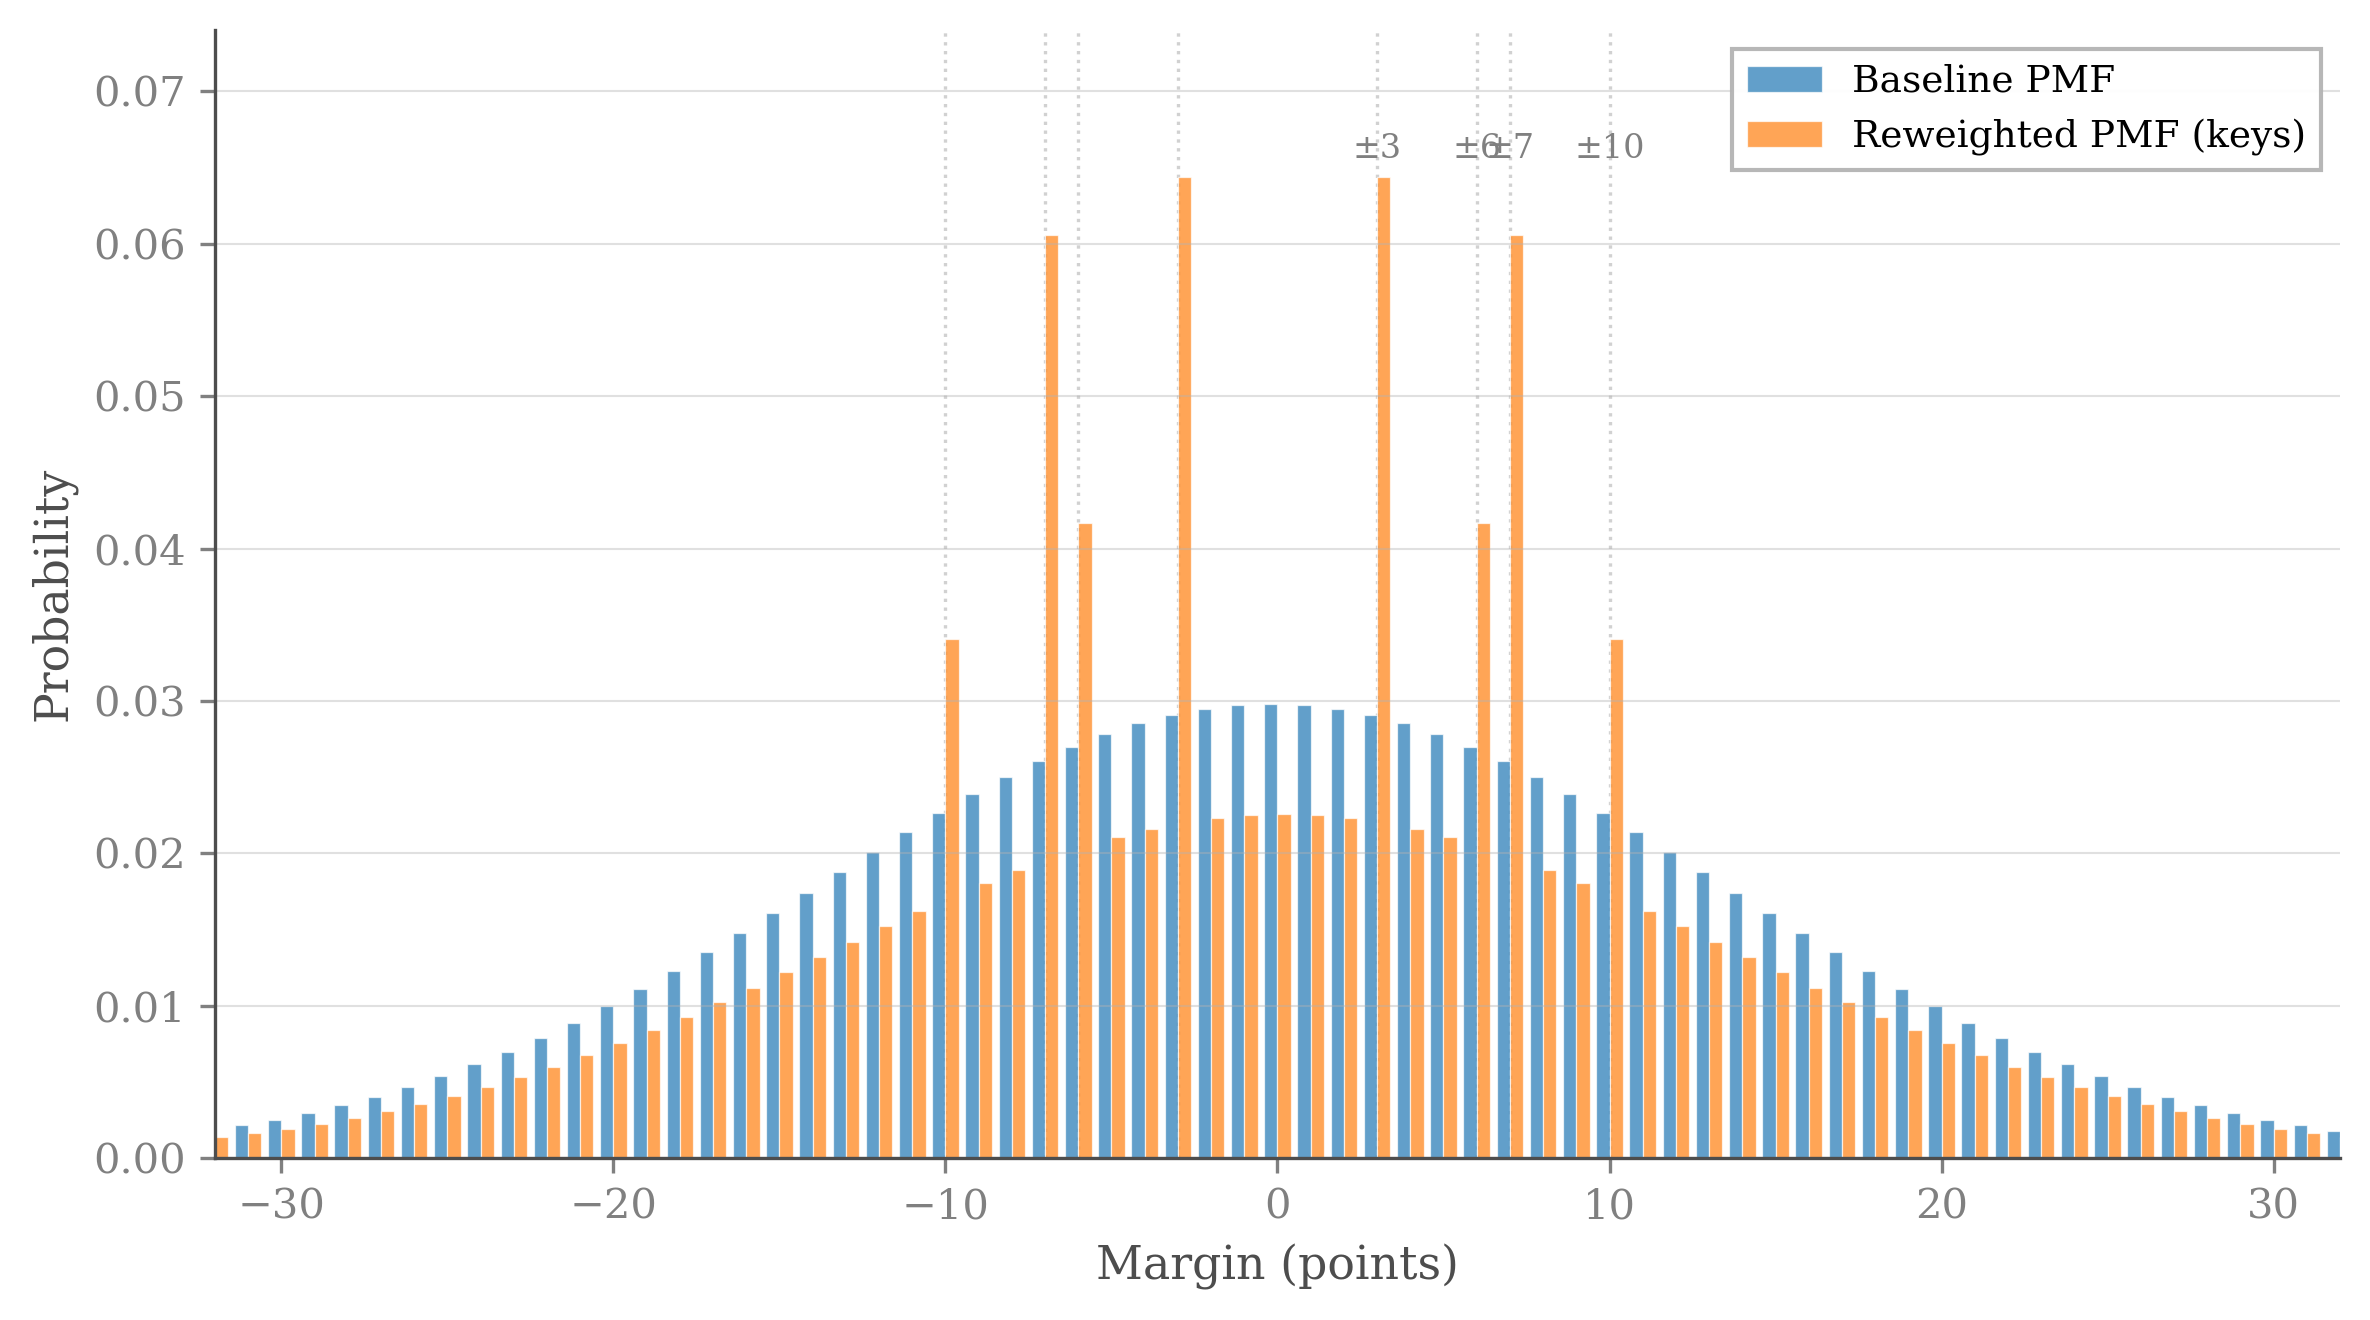
\includegraphics[width=\linewidth]{../figures/key_number_pmf.png}
  \caption[Integer-margin pmf comparison]{Integer-margin pmf comparison. Baseline (e.g., Skellam/discretized Gaussian) vs key-number reweighted distribution matching empirical masses at 3, 6, 7, and 10 while preserving location/scale (\Cref{subsec:key-reweight}).}
  \label{fig:key-pmf}
\end{figure}

\subsection{Teasers and Parlays}
\label{subsec:teasers-parlays}

Teasers (point adjustments for changed odds) and parlays (multiple legs) are common strategy components. We interpret them through joint distributions and correlation risk. A teaser can be attractive when key-number probabilities are underpriced; correlated parlays can be rational when the joint distribution assigns high mass to specific co-movements (e.g., low totals and underdogs). Naive independence assumptions can be severely misleading---motivating the copula-based dependence modeling developed in this chapter.

For the full EV geometry and simulator context, see the teaser surface in \Cref{chap:sim}.

\subsection{Liquidity, Limits, and Execution}
\label{subsec:liquidity}

Modeling performance cannot be divorced from execution. Liquidity varies by book, time to kickoff, and market type. Translating an estimated edge into an executable stake requires accounting for posted limits and depth. Execution-aware evaluation reduces optimism from paper backtests and promotes policies that scale gracefully. The implications for policy evaluation when recommended bets cannot be filled at quoted prices are addressed in \Cref{chap:production}.

%=============================================================================
% CHAPTER SUMMARY
%=============================================================================
\chaptersummary{
This chapter connected classical models (Harville, Stern, Poisson/Skellam, bivariate/dynamic Poisson) with modern machine learning methods (gradient boosting, ensemble theory, SHAP) and emerging approaches (transformers, causal inference, LLMs). We established evaluation tools (CRPS, reliability, conformal prediction) and introduced key-number reweighting and copula-based dependence as recurring motifs. The synthesis emphasizes that a hybrid stack with explicit uncertainty, rigorous calibration, and decision-theoretic staking transforms predictive edge into reliable bankroll growth.
}{
Next we operationalize the data layer that feeds these models: reproducible ingestion, database marts, and feature catalogs (situational, team form, market, roster) in \Cref{chap:data}.
}
